
%%%%%%%%%%%%%%%%%%%%%%%%%%%%%%%%%%%%%%%%%%%%%%%%%%%%%%%%%%%%%%%%%%%%%%%%%
%           Capítulo 3: NOMBRE                   %
%%%%%%%%%%%%%%%%%%%%%%%%%%%%%%%%%%%%%%%%%%%%%%%%%%%%%%%%%%%%%%%%%%%%%%%%%

\chapter{Algoritmos Evolutivos para problemas Multiobjetivo}

Resolver un MOP requeriría obtener todo el conjunto y el frente de Pareto. Sin embargo, esta tarea es muy complicada. Además, debido a que los objetivos frecuentemente se comportan como cajas negras y el espacio de búsqueda es muy grande, obtener el frente de Pareto exacto con algún método algorítmico es frecuentemente una tarea imposible \cite{SMS-EMOA}. 

Una manera de abordar este problema, que es la que usaremos en este trabajo, es encontrar una representación del frente usando individuos de una población que se va iterando para aproximar puntos que cada vez representen más fielmente al frente de Pareto.

El capítulo se organizará de la siguiente forma: en la Sección \ref{sec:QIs} se revisan los indicadores de calidad usados en este trabajo, después, en la Sección \ref{sec:QIs_tax} se explica cómo se clasifican los EMOAs de acuerdo a sus diferentes estrategias, ya sea dentro del algoritmo evolutivo mismo (si son elitistas o no), así como en su mecanismo de selección, etc. Revisaremos con especial cuidado en la Sección \ref{sec:Metodos_QI} aquellos algoritmos que calculan de cada población diversos indicadores de calidad para tener una mejor representación del frente de Pareto (IB-EMOA por sus siglas en inglés), revisando cada uno de los indicadores que usaremos en este trabajo. 

Después, en la Sección \ref{sec:SMS-EMOA} estudiaremos un algoritmos antecedente al usado en este trabajo. El antecedente es el algoritmo prototípico IB-EMOA, llamado SMS-EMOA. Continuaremos con el algoritmo usado en este trabajo en la Sección \ref{sec:PFI-EMOA}. Dicho algoritmo recibe el nombre de PFI-EMOA y fue diseñado para combinar dos indicadores de calidad dentro de su proceso de selección. Finalmente, concluiremos en la Sección \ref{sec:pruebas_estadisticas} con una breve descripción de cómo se comparan diferentes algoritmos entre sí usando pruebas estadísticas.

\section{Indicadores de calidad} \label{sec:QIs}
Al ser un MOP, por definición, un problema que requiere hacer concesiones en cada objetivo, necesariamente habrá varias maneras de comparar dos conjuntos de aproximación para decidir qué conjunto es mejor. La primera de ellas concierne a la dominancia de Pareto entre conjuntos de aproximaciones, siendo esta una extensión del concepto de dominancia entre puntos, como vimos en la Sección \ref{sec:Dominancia_Pareto}. Al extender el concepto a dominancia entre conjuntos, ya no se hace una sólo comparación. Por lo tanto, existen más posibilidades que cubrir, y por ende, más elecciones que tomar. Considerando a dos conjuntos de soluciones $A,B \subseteq \mathbb{R}^m$ en el espacio de objetivos,  veremos algunas manerad de compararlos, definidas en \cite{tesis_mst_guillermo}.

% Se dice que $x$ \textbf{domina débilmente} a $y$, denotado como $x \preccurlyeq y$  si $f_i(x)\leq f_i(y)$ para toda $i\in\{1,\ldots,m\}$; es decir $x$ no es peor (mayor si queremos maximizar o menor si queremos minimizar) que $y$ en ningún objetivo \footnote{Algunas definiciones también piden que $x\neq y$}.  Si además existe un objetivo tal que es peor en alguna dirección, es decir $\exists i \in\{1,\ldots,m\}$ tal que $f_i(x)< f_i(y)$  entonces $x$ \textbf{domina} a $y$, denotado como $x \prec y$. Aún podemos pedir que la relación sea más clara si pedimos $f_i(x)< f_i(y)$, $\forall i \in\{1,\ldots,m\}$. A esta relación se le conoce como \textbf{dominancia estricta}. Esta propiedad dice que una solución es mejor a la otra en todos sus objetivos y se denota como $x \prec \prec y$.


% Una solución $x$ se le llama \textbf{óptima de Pareto} o \textbf{eficiente de Pareto} si no existe ninguna otra solución $y$ tal que $y \prec x$. Es decir si es parte de las mejores soluciones que podemos encontrar. Al conjunto de soluciones eficientes de Pareto se le conoce como \textbf{frente de Pareto}.

% Al intentar definir una única noción de que un conjunto de soluciones sea mejor que otro encontranos, al igual que en la noción de dominancia, que es útil crear definiciones cada vez más estrictas. A continuación se listan algunas de ellas: 

\begin{itemize}
    \item \textbf{Definición 1 (Dominancia Débil)}: Un conjunto \( A \) se dice que domina débilmente a \( B \) si cada solución \( b \in B \) está débilmente dominada por al menos una solución \( a \in A \) y $A\neq B$. Se denota $ A \preceq B$.  Esta es la forma más general y menos restrictiva de las jerarquías entre conjuntos.
    \item \textbf{Definición 2 (Mejor)}: U Se denota a con $ A \vartriangleleft   B$, también conocida como sobredesempeño débil ($A \ \ \mathcal{O}_W \ B$). Es equivalente a decir que $A \preceq B$, pero $B \npreceq A$. En palabras es que $A$ es al menos tan bueno como $B$, mientras que $B$ no es tan bueno como $A$. 
    
    \item \textbf{Definición 3 (Sobredesempeño Fuerte)}: Un conjunto \( A \) se dice que rinde fuertemente a \( B \) si \( A \) domina débilmente a \( B \) y además existe al menos un par de soluciones \( a \in A \) y \( b \in B \) tal que \( a \) domina a \( b \). Denotado $A \ \ \mathcal{O}_S \ B$.
    \item \textbf{Definición 4 (Dominancia)}: Un conjunto \( A \) se dice que domina a \( B \) si cada solución \( b \in B \) está dominada por al menos una solución \( a \in A \). Se denota $A \prec B$. Es importante recalcar que esta medida de dominancia define un orden parcial en el espacio de aproximaciones.
    \item \textbf{Definición 5 (Dominancia Estricta)}: Un conjunto \( A \) se dice que domina estrictamente a \( B \) si cada solución \( b \in B \) está estrictamente dominada por al menos una solución \( a \in A \). Se denota $ A \prec \prec B$, también es llamado sobredesempeño completo $A \ \ \mathcal{O}_C \ B$.
\end{itemize}



Es útil ver las contenciones de las definiciones previas ya que una solución será preferida en este sentido mientras más nos desplazamos hacia el conjunto más pequeño. Así, tenemos 

\begin{align} \label{eq:contencion_comp_sets}
    A \prec \prec B \implies A \prec B &\implies A \ \mathcal{O}_S \ B  \nonumber\\
    \implies A \vartriangleleft B &\implies A\preceq B. \nonumber
\end{align}


En un problema, sin embargo, las nociones de dominancia previamente definidas no se tienen que alinear con todas las preferencias de un tomador de decisiones. Es decir, es posible que un conjunto $A$ que sea, por ejemplo, \textbf{mejor} (en el sentido de la Definición 2) que otro $B$ y que, sin embargo, haya soluciones en $B$ que dominen a algunas de $A$. Para lidiar con estos problemas sería preferible encontrar un conjunto de soluciones que sea una buena representación del frente de Pareto. Así, al preguntarnos qué características son deseables en un algoritmo que busque una representación fidedigna al frente de Pareto encontramos la razón de la construcción de los  \textbf{indicadores de calidad} (QI por sus siglas en inglés).


Con el fin de estudiar propiedades generales de los frentes, se han propuesto categorías de características deseables en la representación del frente:

\begin{itemize}
    \item \textbf{Proximidad o convergencia}: La proximidad que tiene con el frente de Pareto. El tipo de relación que medimos con las definiciones 1 a 5. 
    \item \textbf{Extensión}:  El tamaño de la región que ocupa el conjunto de soluciones. 
    \item \textbf{Uniformidad}: Que tan equidistantes son las soluciones entre sí.
    \item \textbf{Diversidad}: Como extensión y uniformidad suelen intersectar sus objetivos se les suele combinar en la categoría de diversidad, como, por ejemplo, en el estimador de densidad de NSGA-II, explicado en la Sección \ref{sec:nsga2}. 
\end{itemize}

Estos conceptos se  entienden mejor al estudiar la Figura \ref{fig:carac_deseables_aprox}. De las características previamente mencionadas tenemos las siguientes: 

\begin{itemize}
    \item I. tiene buena convergencia y extensión, pero mala uniformidad.
    \item II. tiene bien todo excepto convergencia.
    \item III. tiene muy poca extensión.
    \item IV. tiene todas las características deseables.
\end{itemize}

Incluso intuitivamente, podemos ver que en cada uno de los casos que no son el IV hay deficiencias en las aproximaciones al frente de Pareto. 

\begin{figure}[H]
    \centering
    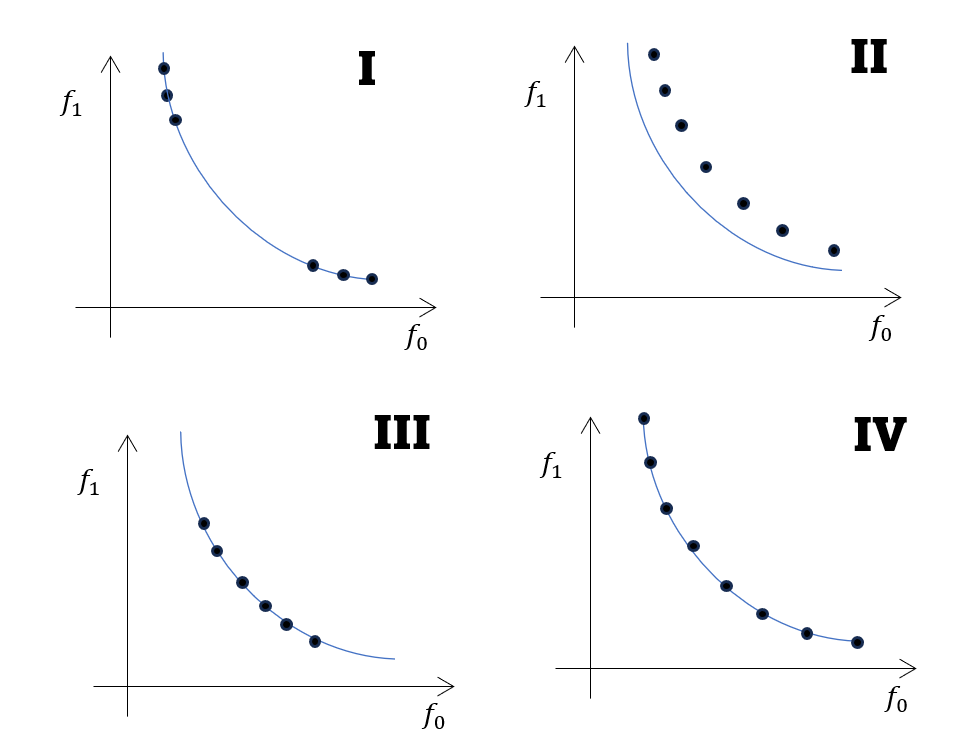
\includegraphics[scale=0.5]{Figuras/carac_deseables_Pareto.png}
    \caption[Características deseables en aproximación al PF]{Características deseables en aproximaciones al frente de Pareto (puntos) y el frente de Pareto como una línea.}
    \label{fig:carac_deseables_aprox}
\end{figure}

Estos indicadores también se pueden clasificar de acuerdo al número de conjuntos de soluciones con los que operan. Si el indicador opera sobre un único conjunto  se le llama un operador unario, mientras que si compara $n$ conjuntos se le llama $n$-ario. Formalmente un indicador $n$-ario \cite{PFI} es  una función que manda  $n$ conjuntos de soluciones a un número real. Es decir $I:\psi_1,\cdots,\psi_n \rightarrow \mathbb{R}$ con $\psi_i \in  \Psi$, el conjunto de aproximaciones, para todo $i$. 


Al ser un mapeo a los números reales, es posible definir un orden total en $\Psi$ a través de un indicador unario. Dicho orden puede coincidir con aquel de la dominancia de Pareto en el siguiente sentido

\begin{equation} \label{eq:consistente_Pareto}
    A \vartriangleleft B \implies I(A) < I(B).
\end{equation}
A esta propiedad del indicador $I$ se le conoce como \textbf{consistencia de Pareto}. Cuando la condición es de desigualdad, es decir 

\begin{equation} \label{eq:consistente_debil_Pareto}
    A \vartriangleleft B \implies I(A)\leq I(B),
\end{equation}

se le llama consistencia débil.

No siempre es posible que nuestro indicador sea consistente de Pareto, por ejemplo, en categorías como diversidad no necesariamente se alinearan los objetivos de esparcir un conjunto con aquellos de encontrar uno menos dominado. Esto se debe a que el esfuerzo de definir indicadores que no sólo traten de dominancia es para no caer en las situaciones donde tratar el problema de esta forma lleva a complicaciones como que el algoritmo se estanque.

A continuación definiremos brevemente los indicadores usados en este trabajo .

\subsection{Hipervolumen} \label{sec:HV}

Se presentó por primer vez en \cite{zitzlerMultiobjectiveOptimizationUsing1998} como una medida del espacio cubierto y se suele abreviar como HV. 
El hipervolumen se construye con un punto de referencia y indica cuál es el tamaño del espacio dominado entre nuestro conjunto y el punto de referencia. Es un operador unario por lo que es muy conveniente usarlo aún cuando no se conoce el frente de Pareto. La sensibilidad de este indicador recae en la elección del punto de referencia; dicho  punto debe ser escogido de manera que sea dominado por todos los puntos del frente. Se puede escoger, por ejemplo, el punto de Nadir, vista en la Definición \ref{def:Nadir}, ya sea sólo o multiplicado por 1.1 para tenerlo un poco alejado. Sin embargo, no hay un consenso de cómo escoger el punto y diferentes puntos de referencia pueden llevar a una evaluación inconsistente \cite{HV_ref_point}. De modo que es importante, al comparar algoritmos, que se establezca una convención del punto de referencia. El hipervolumen es muy usado porque es consistente de Pareto \eqref{eq:consistente_Pareto} y está definido por la siguiente ecuación 

\begin{equation} \label{eq:HV}
    \text{HV}(A)=\lambda\left( \bigcup_{a\in A} \{x|a \prec x \prec r \} \right), \nonumber
\end{equation}
donde $\lambda$ es la medida de Lebesgue y mide el hipervolumen de la unión de los hipercubos definidos por cada una de las soluciones $a$ que viven en $A$ y el punto de referencia $r$. Así para cada uno de los conjuntos, los puntos $x$ serían aquellos que están entre el punto de la solución $a$ y el pinto de referencia $r$. Como podemos ver en la Figura \ref{fig:HV}.

\begin{figure}[H]
    \centering
    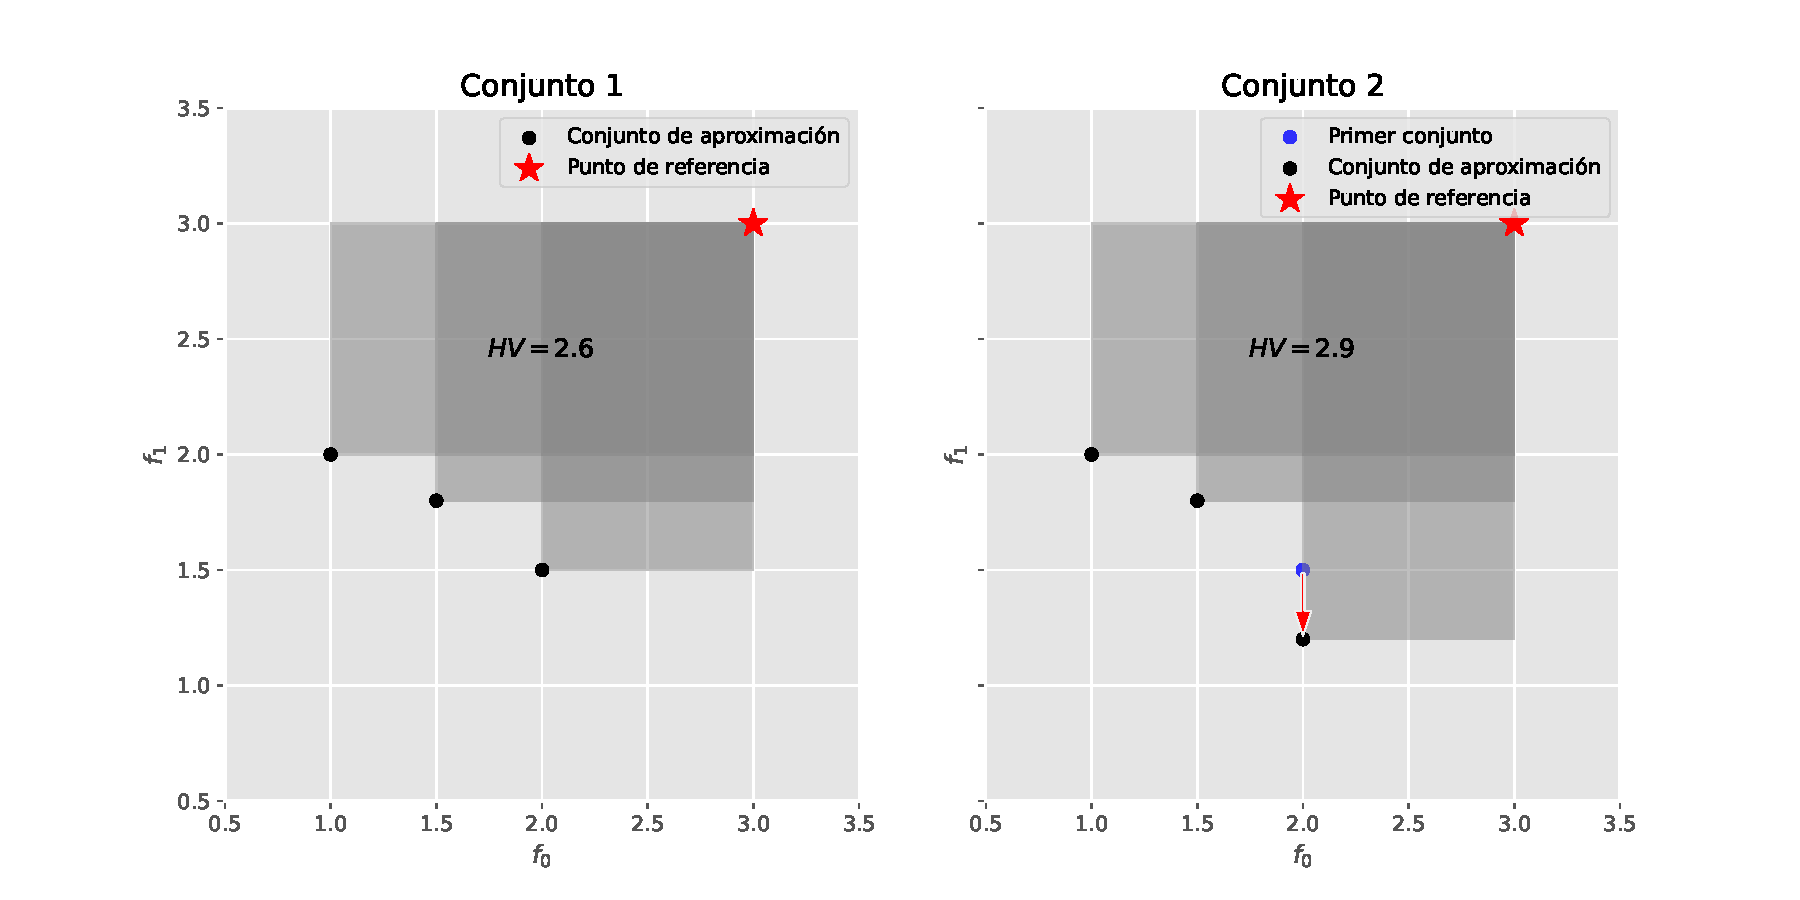
\includegraphics[scale=.6]{./Figuras/HV_demo.pdf} 
    \caption[Hipervolumen]{Cálculo del indicador HV para dos conjuntos, podemos ver su espacio dominado. Del lado derecho movemos sólo un punto hacia un menor $f_1$ y vemos que el HV toma en cuenta este aumento.}
    \label{fig:HV}
\end{figure}

Otra característica deseable de este indicador es que se probó en \cite{Measure_Pareto_Optima} que para un espacio de búsqueda finito y un punto de referencia, la maximización del hipervolumen equivale a encontrar el conjunto de Pareto. 

\subsection{Distancia Generacional (GD)} \label{sec:GD}
Este es un indicador binario en el que asumimos que tenemos un conjunto de referencia, idealmente este conjunto es la mejor representación del frente de Pareto posible. Fue introducido en \cite{GD}.

La idea del indicador es simplemente medir la distancia entre un conjunto de aproximación $\mathcal{A}$, que produciríamos con un algoritmo, al conjunto de referencia $\mathcal{Z}$. Así obtenemos la siguiente ecuación.

\begin{equation} \label{eq:GD}
    \text{GD} \left( \mathcal{A},\mathcal{Z} \right) = \frac{1}{|\mathcal{A}|} \sum_{x\in A} d_{\min}(x,Z)
\end{equation}

donde $d_{\min}(x,Z)=\min_{z \in \mathcal{Z}}{d(x,z)}$, con $d(x,y)$ una función de distancia, por ejemplo la norma euclidiana usual. En la Figura \ref{fig:GD_demo} podemos observar los conjuntos de aproximación $A$ y $B$ y los puntos mínimos con los que se calcula $d_{\min}$. Vemos que el conjunto $B$ al ser cercano a un punto del conjunto de referencia tiene un menor $\text{GD}$ que $A$.

\begin{figure}[H]
    \centering
    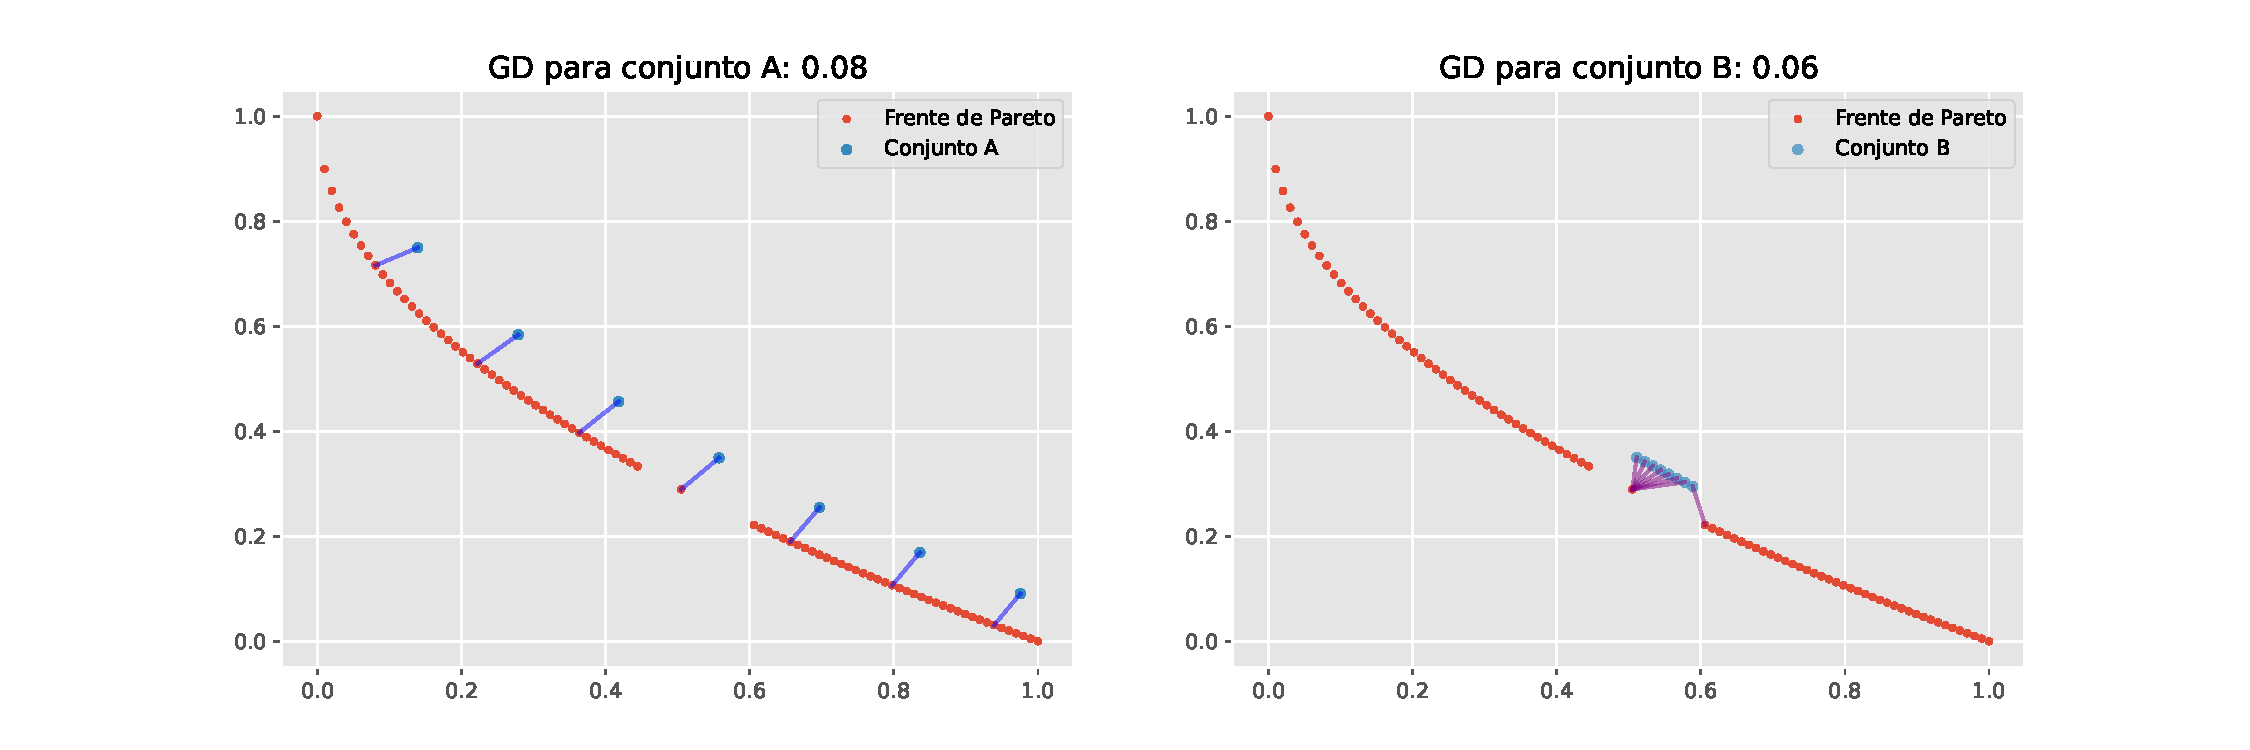
\includegraphics[width=\textwidth]{Figuras/GD_demo.pdf}
    \caption[GD]{Ilustración del cálculo del indicador GD para dos conjuntos.}
    \label{fig:GD_demo}
\end{figure}

\subsection{Distancia Generacional Invertida (IGD)} \label{sec:IGD}
Propuesta por primera vez en \cite{IGD}, la distancia generacional (IGD) invertida mide la distancia del $\mathcal{Z}$ de referencia al conjunto de aproximación, es decir sólo intercambiamos $\mathcal{A}$ y $\mathcal{Z}$ con respecto a la Ecuación \ref{eq:GD}.

\begin{equation} \label{eq:IGD}
    \text{IGD}(A,\mathcal{Z})=\frac{1}{|\mathcal{Z}|}\sum_{z\in\mathcal{Z}} d_{\min}(z,\mathcal{A}), \nonumber
\end{equation}
donde $d_{\min}(x,Z)=\min_{z \in \mathcal{Z}}{d(x,z)}$, con $d(x,y)$ una función de distancia. Esta definición permite tratar casos que GD favorecería y que usalmente no cumplen con requisitos como la diversidad. En la Figura \ref{fig:IGD_demo} vemos la diferencia de calcular ambos indicadores para los mismos conjuntos que en \ref{fig:GD_demo}. En particular, notamos cómo IGD si distingue entre ambos conjuntos, teniendo un valor más pequeño para el conjunto que tiene mejor diversidad.

\begin{figure}[H]
    \centering
    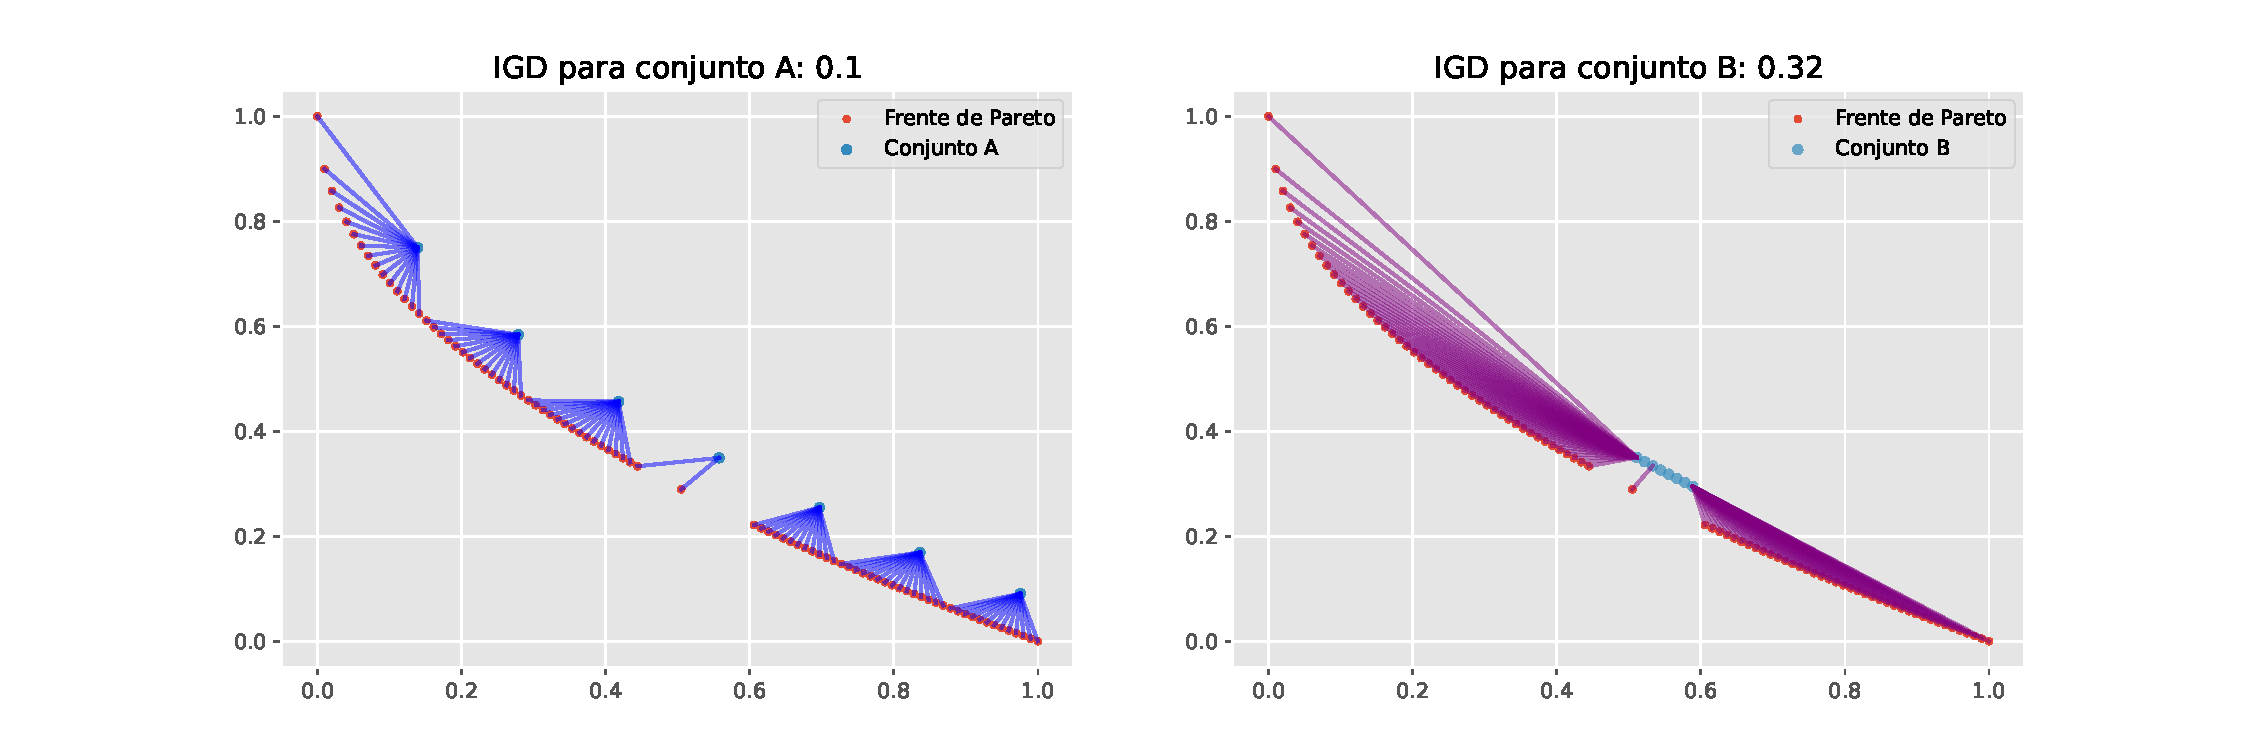
\includegraphics[width=\textwidth]{Figuras/IGD_demo.pdf}
    \caption[IGD]{Ilustración del cálculo del indicador IGD para dos conjuntos.}
    \label{fig:IGD_demo}
\end{figure}


\subsection{Distancia Generacional Invertida + (IGD +)} \label{sec:IGDp}
Definido en \cite{ishibuchiModifiedDistanceCalculation2015}, y denotado como IGD+, es una variación del indicador IGD en donde se usa una función de distancia euclidiana modificada dentro del cálculo del promedio. Si denotamos como $Z$ al conjunto de soluciones, $A$ al conjunto de al frente de Pareto, La ecuación tiene una forma similar a la de IGD usual, la diferencia es que usa la siguiente definición de distancia entre el conjunto de referencia y el de aproximación, dada por $$d^{+}(\vec{a},\vec{z})=\sqrt{\sum_{i=1}^m \max(a_i-z_i,0)^2} $$

Entonces la ecuación para el indicador queda como

\begin{equation} \label{eq:IGDp}
    \text{IGD}^+(A,Z) =  \frac{1}{|Z|} \sum_{\vec{z}\in Z}\min_{\vec{a}\in A} d^{+}(\vec{a},\vec{z}).
\end{equation}


Esta modificación hace al indicador uno débilmente consitente de Pareto (definido en la Ecuación \ref{eq:consistente_debil_Pareto}) que como hemos mencionado es una propiedad deseable de un indicador de convergencia. Regresando a la Ecuación \ref{eq:IGDp}, como $\vec{a}$ pertenece al conjunto de referencia y $\vec{z}$ al de aproximación, la Ecuación \ref{eq:IGDp} indica que, por cada dimensión, si la aproximación $z_i$ domina a la solución $a_i$ se calcula la distancia euclidiana usual. En caso contrario se calcula la distancia entre la aproximación $z$ y la región dominada de la referencia $a$. Al ser una medida de distancia, es mejor mientras sea más pequeña. En la Figura \ref{fig:comp_IGD_IGDp} podemos ver dos conjuntos distintos  en el que el conjunto $B$ incluso domina al conjunto de referencia, sin embargo, IGD nos diría que el conjunto $A$ es mejor al tener un menor valor del indicador. Con la modificación dada por la Ecuación \ref{eq:IGDp}, el indicador puede identificar que el conjunto $B$ domina al conjunto $A$.

\begin{figure}[H]
    \centering
    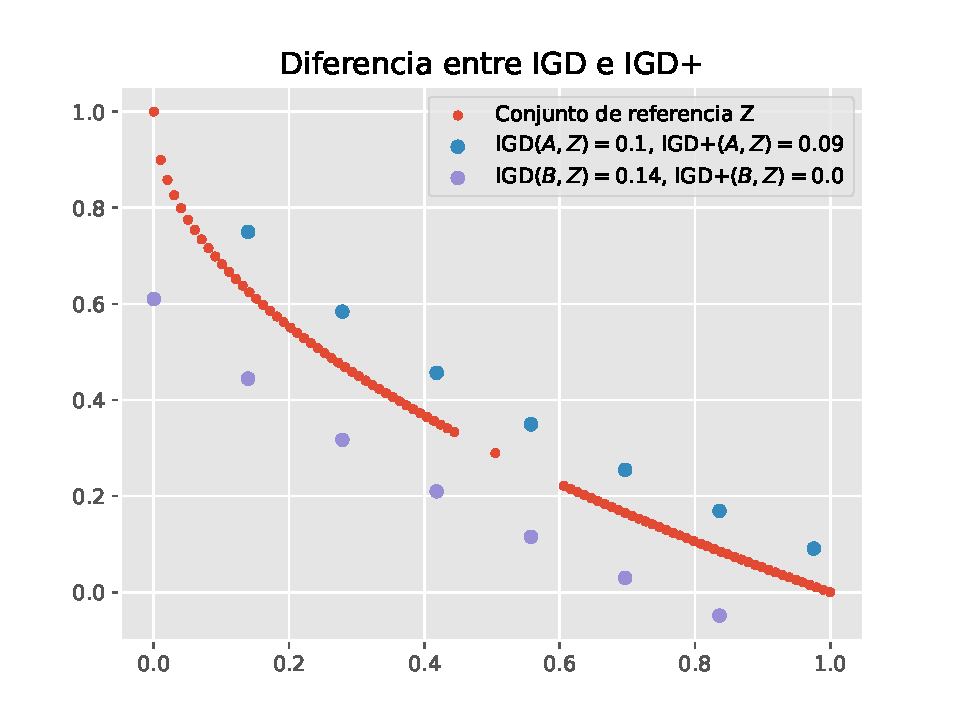
\includegraphics[width=0.8\textwidth]{./Figuras/igdp_demo.pdf} 
    \caption[IGD vs IGD+]{Comparativa entre IGD usual e IGD$+$.}
    \label{fig:comp_IGD_IGDp}
\end{figure}

\subsection{Epsilon +} \label{sec:Epsilonp}
Escrito como $\epsilon_+$ \cite{epsilonplus} es un indicador binario que mide la distancia mínima que habría que recorrer un conjunto $A$ para dominar débilmente al conjunto $B$, la siguiente ecuación describe el cálculo del indicador

\begin{equation} \label{eq:epsp}
    \epsilon_+(A,B)= \max_{b\in B} \min_{a\in A}\max_{j\in 1,\ldots, m} a_j-b_j. 
\end{equation}

Donde $A$ y $B$ son usualmente el conjunto de referencia y el de aproximación. De la Ecuación \ref{eq:epsp} vemos que el indicador depende del orden de los conjuntos.
Para explicar de manera más clara que hace este indicador miremos la Figura \ref{fig:epsp}. Vemos que después de trasladar $A$ por $\epsilon+$ el conjunto $A$ domina al conjunto de referencia. Así, el objetivo de este indicador es minimizar el traslado que hay que hacer para tener similitud entre la referencia y la aproximación. Al requerir un conjunto de referencia, la eficacia del indicador dependerá de si tenemos una buena aproximación al frente de Pareto. 

\begin{figure}[H]
    \centering
    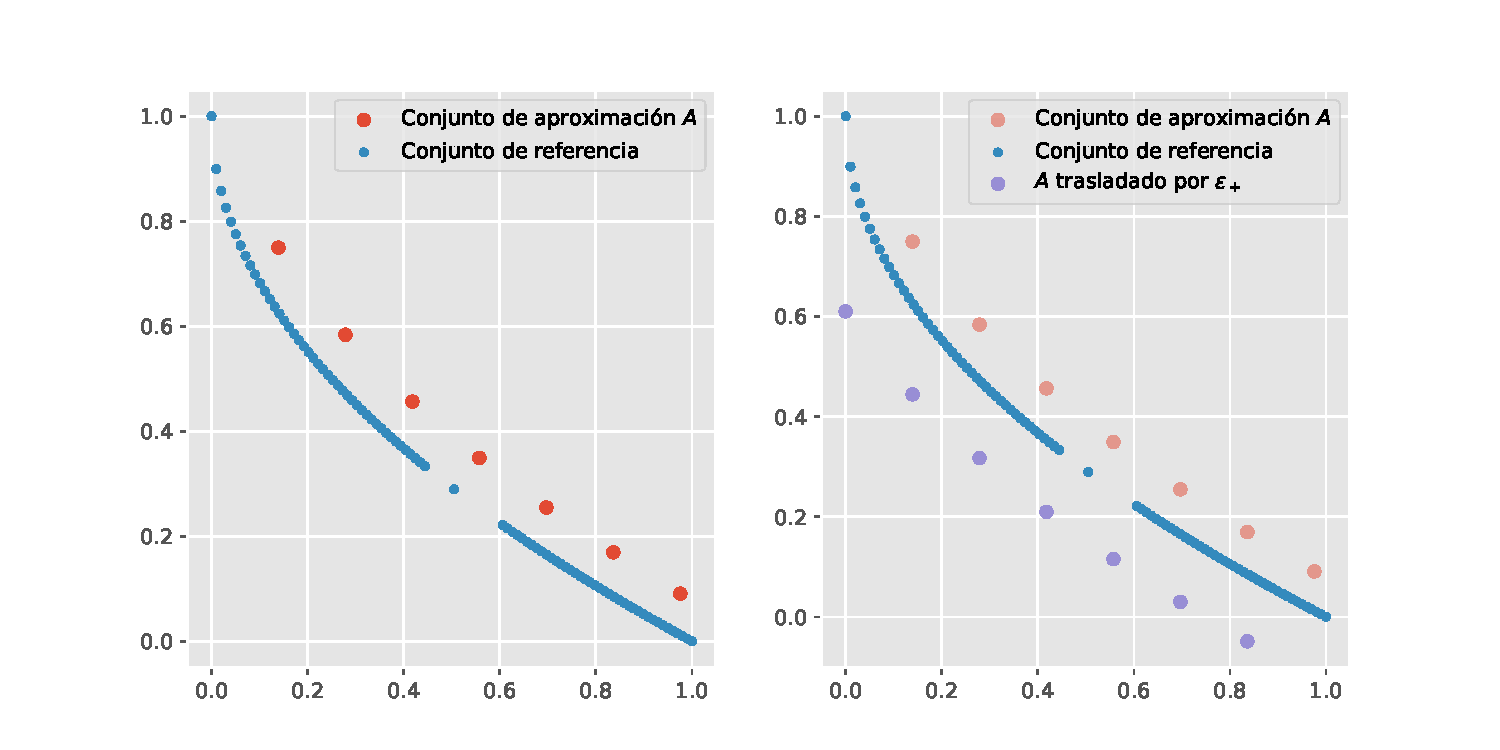
\includegraphics[width=\textwidth]{Figuras/epsilon_plus_demo.pdf}
    \caption[$\epsilon+$]{Ilustración del valor del indicador $\epsilon_+$.}
    \label{fig:epsp}
\end{figure}

\subsection{Diversidad de Solow-Polasky (SPD)} \label{sec:SPD} 
El indicador de diversidad de Solow-Polasky (SPD por sus siglas en inglés) fue originalmente creado en el contexto de biología para medir diversidad de especies y ha sido adaptado para su uso en problemas multiobjetivo. Esto se debe a que satisface propiedades deseables de operadores de diversidad \cite{SPD} como monoticidad en variedades, en distancia y que se mantengan constantes al agregar un elemento que ya esté presente en el conjunto de soluciones.

Dada una población $P = \{P_1, \ldots, P_\mu\}$ de $\mu$ individuos y distancias por pares $d(P_i, P_j)$ para $1 \leq i,j \leq \mu$, Definimos la matriz $M$ de ($\mu \times \mu$) como $M_{ij} = \exp(-\theta  d(P_i, P_j))$. Así, el indicador queda definido por la siguiente ecuación:

\begin{equation} \label{eq:SPD}
    D_{SP}(P) = \sum_{1 \leq i,j \leq \mu} M_{ij}^{-1} \in [1, \mu], \nonumber
\end{equation}


donde $M^{-1}$ es la inversa generalizada de Moore-Penrose de la matriz $M$. Puede ser interpretado como el número de especies diferentes en la población. Su valor cae en los reales entre $1$ y $\mu$ por lo que nos da una medida fina de diversidad. En la Figura \ref{fig:SPD}, podemos ver diferentes valores de SPD para cien puntos distribuidos de diferente manera en el círculo unitario. Vemos que aquellos menos concentrados en el origen reciben mayor SPD. 

\begin{figure}[H]
    \centering
    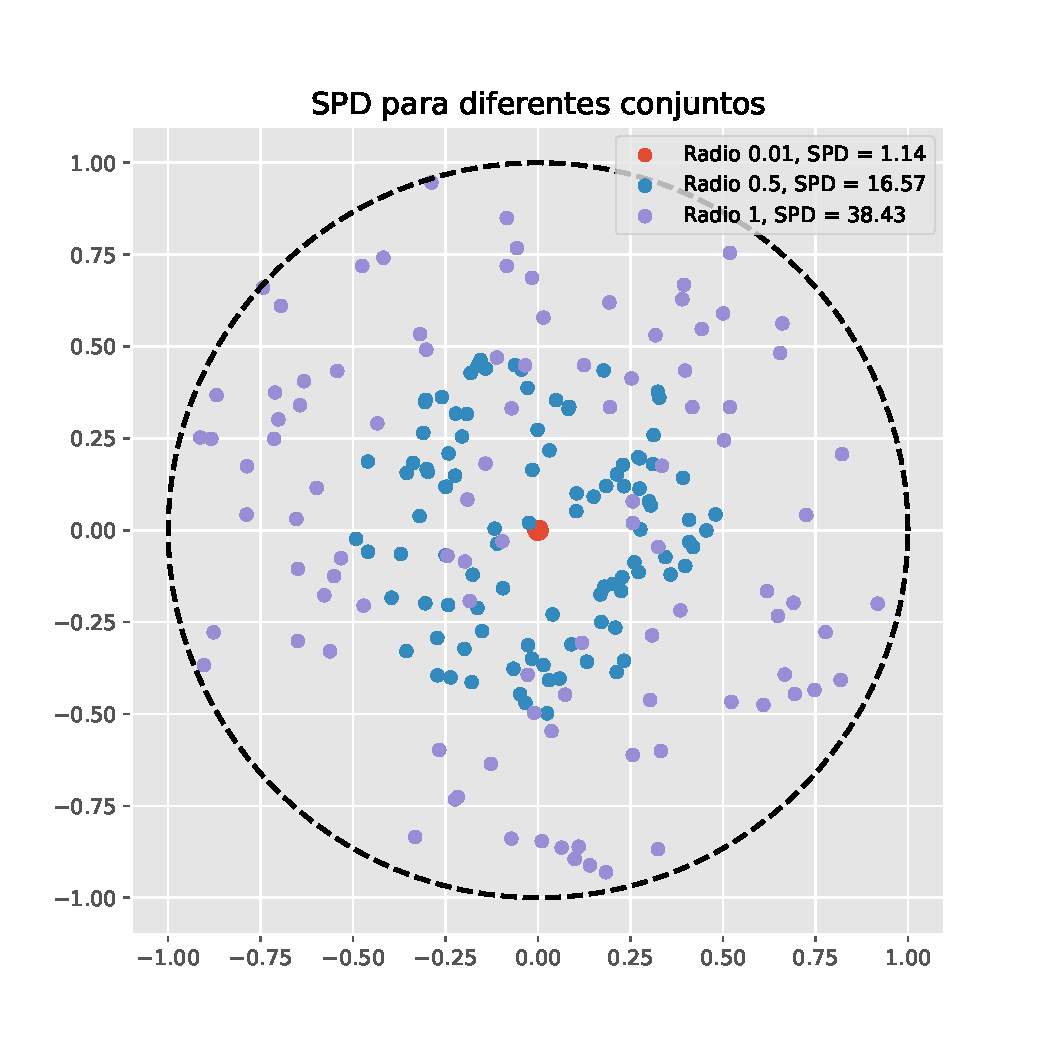
\includegraphics[scale=0.7]{../Figuras/SPD_demo.pdf}
    \caption[SPD]{Valores de SPD para diferentes distribuciones de puntos en el circulo unitario.}
    \label{fig:SPD}
\end{figure}


% The Solow-Polasky diversity indicator is a measure of the diversity of a set of points or solutions, based on a utilitarian model of species conservation². It is defined as the sum of the inverse of the correlation matrix of the points, where the correlation function is exponential⁷. The Solow-Polasky diversity indicator is to be **maximized** to obtain a more diverse set⁷. A higher value of the indicator means that the points are more different from each other and cover a larger area in the space. A lower value means that the points are more similar and clustered together. Therefore, if you want to optimize the Solow-Polasky diversity indicator, you should aim for a **maximal** value.

% Source: Conversation with Bing, 10/21/2023
% (1) A Survey of Diversity Oriented Optimization: Problems, Indicators, and .... https://link.springer.com/chapter/10.1007/978-3-319-49325-1_1.
% (2) indicator — Useful diversity indicators — diversipy 0.7 documentation. https://ls11-www.cs.tu-dortmund.de/people/swessing/diversipy/doc/indicator.html.
% (3) solow_polasky : Solow-Polasky measure - R Package Documentation. https://bing.com/search?q=solow+polasky+diversity+indicator.
% (4) solow_polasky : Solow-Polasky measure - R Package Documentation. https://rdrr.io/github/jakobbossek/ecr3vis/man/solow_polasky.html.
% (5) Diversity-Indicator Based Multi-Objective Evolutionary Algorithm: DI .... https://link.springer.com/chapter/10.1007/978-3-030-12598-1_28.
% (6) Defining and Optimizing Indicator-based Diversity Measures in .... https://bin.re/files/pdf/3.pdf.
% (7) Two-objective solution set optimization to maximize hypervolume and .... https://ieeexplore.ieee.org/document/6505243.

\subsection{R2} \label{sec:R2}
El indicador $R2$ pertenece a un conjunto más general de indicadores conocido como la familia $R$ \cite{R2}. Integra las preferencias del tomador de decisiones mediante una función de densidad de utilidad $h(u)$ y compara un conjunto de aproximación $\mathcal{A}$ con uno de referencia $\mathcal{Z}$ mediante la siguiente ecuación

\begin{equation} \label{eq:R2_completo}
    R2(\mathcal{Z},\mathcal{A},U)=\int_{u\in U} h(u)u^*(\mathcal{Z}) dU- \int_{u\in U} h(u) u^*(\mathcal{Z})du, 
\end{equation}
donde  $u^*(\mathcal{A})$ es el mejor valor que se logra en el conjunto $A$ dado esta función de utilidad. Cuando la información sobre la preferencia del tomador de decisiones no se conoce se puede suponer una función uniforme sobre las funciones de utilidad. Si el conjunto de funciones de utilidad es discreto se puede cambiar la integral por una suma. Además, al comparar el $R2$ de dos conjuntos distintos, podemos ver que el segundo término de \ref{eq:R2_completo} se cancela en la diferencia. De modo que bajo estas características tenemos

\begin{equation} 
    R2(\mathcal{A})=\frac{1}{|W|}\sum_{w\in W} h(u)u(\mathcal{A},w), \nonumber
\end{equation}

$W$ es un conjunto de pesos\\
$h(u)$ es una función de densidad sobre las funciones de utilidad\\
$u(\mathcal{A},w)$ es una función de utilidad.

para la función $u(\mathcal{A},w)$ se pueden usar escalarizaciones comunes como suma ponderada \eqref{eq:suma_ponderada} o la función de escalarización de Tchebycheff \eqref{eq:tchebychev}. Este indicador tiene la ventaja de tener un costo computacional relativamente pequeño, pero tiene menor precisión que otros indicadores que consideran un conjunto continuo de pesos como el IPF. 

% Además cumple con las siguientes características \cite{tesis_phd_guillermo}

% \begin{itemize}
%     \item Es débilmente monótono, i.e.,
% \end{itemize}
% IR2(A)  IR2(B) en caso de que A  B, (2) simultaneamente evalua todos los aspectos
% deseables de una aproximacion al frente de Pareto, (3) las soluciones que genera
% estan usualmente uniformemente distribuidas, y (4) es mucho menos costoso computacionalmente
% que HV.

En este trabajo usamos un conjunto de funciones de utilización conocidas como ASF (Achievement Scalarizing Function) que están dadas en función un conjunto de vectores de pesos convexos\footnote{Los vectores convexos, son no negativos $\lambda_i\geq 0, \forall i$ y suman a uno $\sum_i \lambda_i =1$} $\Lambda$ y un vector de referencia $z$. 

\begin{equation}\label{eq:R2}
    R2(\mathcal{A}, \Lambda, \mathbf{z}) = \frac{1}{|\Lambda|} \sum_{\mathbf{\lambda} \in \Lambda} \max_{\mathbf{a} \in \mathcal{A}} \left\{ \max_{i \in \{1, \ldots, m\}} \lambda_i \left\{ |a_i - z_i|\right\} \right\}
\end{equation}

La región definida por los vectores convexos forman un simplejo en $\mathbb{R}^m$. Los puntos de ese simplejo definirán las funciones de utilidad que evaluamos en \ref{eq:R2}. Existen métodos para distribuir estos puntos como SLD (Simple Latex Desing). En este trabajo usamos un método definido para maximizar la Energía-S de Riesz de los vectores en el simplejo. 

% En la Figura \ref{fig:R2} vemos el cálculo del indicador R2, los vectores de pesos que nos ayudan a materializar las preferencias de la función de utilidad.

% \begin{figure}[H]
%     \centering
%     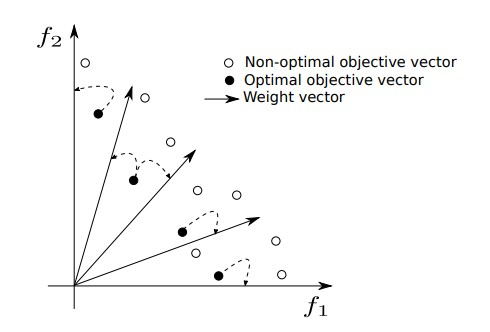
\includegraphics[scale=.6]{./Figuras/R2.jpg} 
%     \caption[R2]{Cálculo de R2. Imagen tomada de \cite{tesis_mst_guillermo}.}
%     \label{fig:R2}
% \end{figure}

% The R2 indicator is a measure of the quality of a set of solutions in multiobjective optimization, based on a utilitarian model of species conservation². It is defined as the weighted sum of the hypervolumes of the scalarized optimization problems⁶. The R2 indicator is to be **maximized** to obtain a better set of solutions⁴⁵. A higher value of the R2 indicator means that the solutions are more optimal and diverse, and cover a larger portion of the Pareto front. A lower value means that the solutions are less optimal and diverse, and cover a smaller portion of the Pareto front. Therefore, if you want to optimize the R2 indicator in multiobjective optimization, you should aim for a **maximal** value.

% Source: Conversation with Bing, 10/21/2023
% (1) . https://bing.com/search?q=R2+indicator+in+multiobjective+optimization.
% (2) undefined. https://arxiv.org/abs/2305.11774.
% (3) R2-IBEA: R2 indicator based evolutionary algorithm for multiobjective .... https://ieeexplore.ieee.org/document/6557783/.
% (4) R2-EMOA: Focused Multiobjective Search Using R2-Indicator-Based Selection. https://inria.hal.science/hal-00807901/document/.
% (5) A new weight vectors generation method for R2 indicator based .... https://ieeexplore.ieee.org/document/7979300/.
% (6) Multi-objective particle swarm optimization with R2 indicator and .... https://link.springer.com/article/10.1007/s40747-021-00445-3.
% (7) undefined. https://ieeexplore.ieee.org/servlet/opac?punumber=6552460.

\subsection{Energía S} \label{sec:Energía-S}
La Energía-S de Riesz \cite{sEnergy} es una medida de la uniformidad de soluciones que depende de un parámetro $s$. Está basada en que la energía potencial entre dos cuerpos va como el inverso de su distancia.  Tiene la ventaja de no necesitar un conjunto de referencia, es decir, es un operador unario y está dada por 

\begin{equation} \label{eq:S_energy}
    E_s(A)=\sum_{i\neq j} ||a_i-a_j||^{-s},
\end{equation}
mientras $s\rightarrow \infty$ la Energía-S de Riesz tiende a soluciones más uniformes. Además, el parámetro $s$ es independiente de la forma y ha sido usado para producir conjuntos uniformemente distribuidos en una clase grande de variedades $d$-dimensionales rectificables.

% Conjuntos con diferente energía S comparados con conjuntos con diferente SPD. 



\subsection*{Contribución de solución al indicador}
Para la siguiente sección también será útil definir la contribución de una solución a un cierto indicador; es decir, que tan importante es la solución particular para el desempeño de la solución. Eso es útil porque podemos distinguir cuál es la solución que menos ayuda a optimizar un indicador dado. De manera más formal usamos la Ecuación \eqref{eq:Contribucion}. Esta mide el efecto de quitar un punto en el cálculo del indicador y ver su efecto. Si $a$ es un punto que ayuda mucho a elevar el indicador, entonces $I(A)$ será muy diferente a $I(A \setminus \{a\})$.

\begin{equation} \label{eq:Contribucion}
    C_I(a,A)=|I(A)-I(A \setminus \{a\}) |.
\end{equation}


\section{Taxonomía de EMOAs} \label{sec:QIs_tax}

En esta sección se revisa una clasificación de EMOAs además de dar un ejemplo de cada uno de ellos. Las categorías que se revisan son: 

\begin{itemize}
\item No-Elitistas no-basados en optimalidad de Pareto. Poniendo como ejemplo a VEGA \cite{schafferMultipleObjectiveOptimization1984}.
\item No-Elitistas basados en dominancia de Pareto. Poniendo como ejemplo a NSGA \cite{debFastElitistNondominated2000}.
\item Elitistas basados en dominancia de Pareto. Poniendo como ejemplo a NSGA-II \cite{seifbarghyNovelMetaheuristicAlgorithm2016}.
\item EMOAs basados en indicadores. Poniendo como ejemplo a SMS-EMOA \cite{SMS-EMOA}.
\end{itemize}


\subsection*{No-Elitistas no-basados en optimalidad de Pareto} \label{sec:VEGA}

Para ejemplificar esta clase de algoritmos explicaremos el primer EMOA propuesto por Schaeffer \cite{schafferMultipleObjectiveOptimization1984} llamado VEGA (Vector Evaluation Genetic Algorithm). Este algoritmo consiste en dividir la población total de $M$ individuos en subpoblaciones y hacer que cada uno de ellos evolucionara para resolver uno de los $k$ objetivos en un algoritmo no-elitista. Después en la siguiente generación, se revolvían de manera aleatoria los individuos y se volvían a dividir en subpoblaciones para atacar cada uno de los objetivos que, para cada individuo, podría ser un objetivo distinto al que se le había asignado previamente, podemos ver una representación en la Figura \ref{fig:VEGA}, adaptada de \cite{coelloEvolutionaryAlgorithmsSolving}.

\begin{figure}[H]
    \centering
    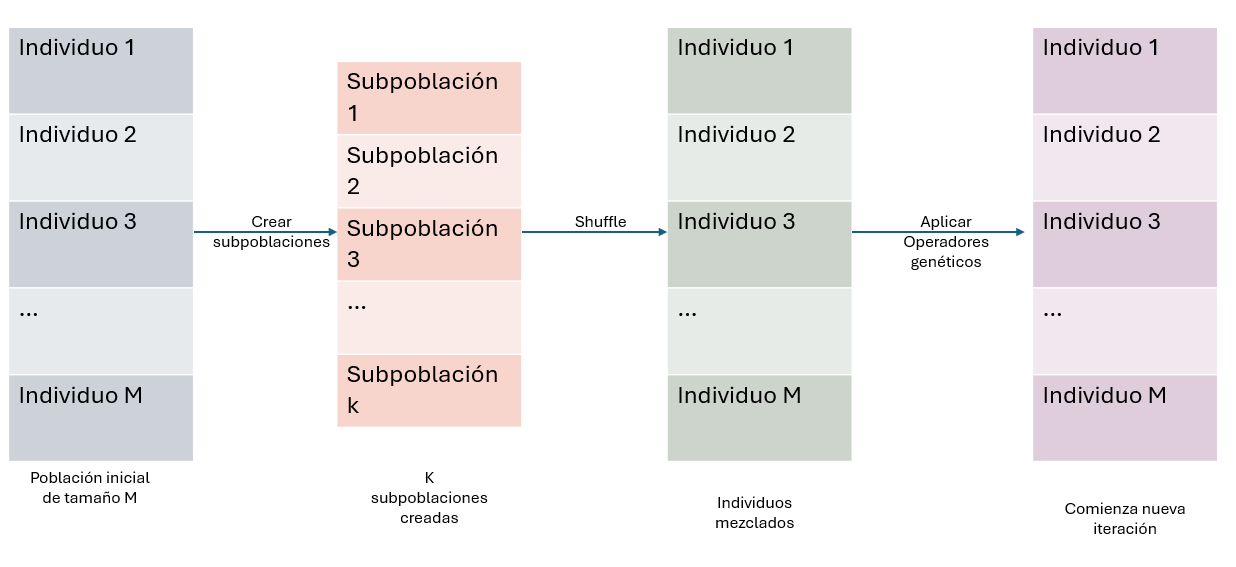
\includegraphics[width=\textwidth]{Figuras/VEGA_diagrama.png}
    \caption[VEGA]{Ilustración del algoritmo de VEGA.}
    \label{fig:VEGA}
\end{figure}

Este algoritmo presentó problemas para encontrar diversidad y para encontrar soluciones que realmente no fueran óptimas de Pareto. Además, el enfoque de cada subpoblación en objetivos llevó a lo que Schaeffer llamó especiación, en el que se seleccionan individuos que son muy buenos para una tarea y malos para las demás, de modo que se obtiene un desempeño aceptable, pero no excelente. Este algoritmo no integra específicamente la dominancia de Pareto por lo que se puede clasificar como uno \textbf{No elitista no basado en optimalidad de Pareto}.

\subsection*{No-Elitistas basados en dominancia de Pareto}

Para ejemplificar este tipo de algoritmos se describirá brevemente uno de los más importantes dentro de esta categoría, NSGA. En 1994 se presentó el algoritmo Nondominated Sorting Genetic Algorithm \cite{srinivasMuiltiobjectiveOptimizationUsing1994} que ataca directamente el problema de obtener soluciones no dominadas mediante una clasificación de capas de subpoblaciones. Se realiza un procedimiento iterativo en el que se seleccionan los individuos que no estén dominados y se les asigna un ranking de 1, después se quitan estos individuos de la población y se repite el procedimiento hasta agotar los individuos incrementando el ranking en cada capa, como se puede ver en la Figura \ref{fig:nsga1}.

\begin{figure}[H]
    \centering
    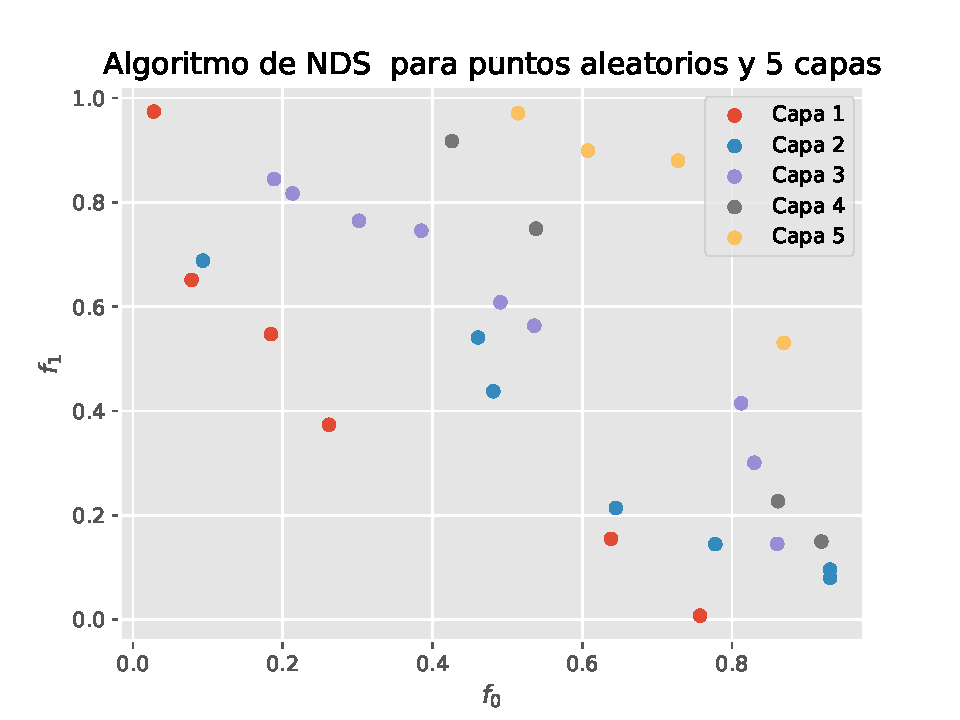
\includegraphics[width=\textwidth]{Figuras/nds.pdf}
    \caption[NSGA]{Capas del algoritmo de NSGA. Primero se encontrarían aquellos que están etiquetados como rank 1, se quitarían de la población y así sucesivamente.}
    \label{fig:nsga1}
\end{figure}

% ¿Hace Falta poner algoritmo?

Este algoritmo también es no-elitista lo que hace muy costoso el cálculo de los rankings en cada una de las generaciones por lo que se le llama un algoritmo \textbf{No-elitista basado en optimalidad de Pareto}.

\subsection*{Elitistas basados en dominancia de Pareto.} \label{sec:nsga2}

Para ejemplificar este tipo de algoritmos se explica brevemente el funcionamiento del algoritmo NSGA-II.  

En el 2000 se publicó \cite{debFastElitistNondominated2000} una actualización del algoritmo anterior que ataca el problema de la complejidad computacional y el de la diversidad de las soluciones proponiendo dos mecanismos diferentes. Para el problema de la complejidad ahora se usa un enfoque elitista. De esta forma se pueden conservar rankings de generaciones anteriores y no se tiene la carga computacional de estarlos calculando constantemente. Además de esto para asegurar que los individuos de una población no se concentran en una región pequeña del espacio, se suelen usar algún \textbf{estimador de densidad} que mide que tan cerca están los puntos y puede lograr que no existan demasiados aglomerados en una región pequeña del espacio. En NSGA-II se usa un estimador de densidad llamado \textbf{crowding distance} en su operador de selección para calcularlo, primero se ordenan los valores de los objetivos en cada una de las direcciones. A los puntos extremos en este ordenamiento se les asigna una distancia infinita porque no se quiere que se eliminen de la población. Para el individuo $i$-ésimo se realiza el siguiente cálculo

\begin{equation} \label{eq:crowding_distance}    
    \text{crowding distance} (d_i) = \sum_{m=1}^M \left( \frac{f_m^{(i+1)} - f_m^{(i-1)}}{f_m^{\text{max}} - f_m^{\text{min}}} \right)
\end{equation}

donde:
\begin{itemize}
    \item \(d_i\) es la \text{crowding distance} para el individuo \(i\).
    \item \(M\) es el número de objetivos.
    \item \(f_m\) representa la función objetivo \(m\).
    \item \(f_m^{(i+1)}\) y \(f_m^{(i-1)}\) son los valores de la función objetivo \(m\) de los individuos adyacentes a \(i\) en la lista ordenada.
    \item \(f_m^{\text{max}}\) y \(f_m^{\text{min}}\) son los valores máximos y mínimos de la función objetivo \(m\) entre todos los individuos.
\end{itemize}

Este operador mide el perímetro del cuadrado que separa a una solución de sus vecinos más cercanos en todas direcciones, como podemos ver en la Figura \ref{fig:crowding_distance}.  Cuando existe algún empate en el rango de dos soluciones, la solución que tenga mayor crowding distance es preferida. De este modo se promueve que la densidad de las soluciones sea menor y esto ayuda a la diversidad de la población. 

\begin{figure}[H]
    \centering
    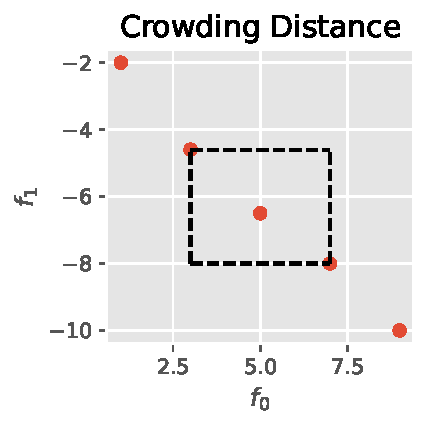
\includegraphics[scale=1]{./Figuras/crowding_distance.pdf}
    \caption{Vemos el rectángulo con el que se calcula la crowding distance de la solución de enmedio.}
    \label{fig:crowding_distance}
\end{figure}

\begin{algorithm}
    \caption{Algoritmo NSGA-II}
    \begin{algorithmic}[1]
    \setlength{\itemsep}{1pt} % Set the spacing between items
\setlength{\parskip}{0pt} % Set paragraph spacing to zero
    \State $P_0 \gets \text{InicializarPoblación()}$
    \State $t \gets 0$
    \While{\text{Criterio de Terminación NO CUMPLIDO}}
        \State $Q_t \gets \text{OperacionesGenéticas}(P_t)$
        \State $R_t \gets P_t \cup Q_t$
        \State $\{F_1, F_2, \ldots\} \gets \text{NDS}(R_t)$
        \State $P_{t+1} \gets \text{vacío}$
        \State $i \gets 1$
        \While{$|P_{t+1}| + |F_i| \leq N$}
            \State $\text{CrowdingDistance}(F_i)$
            \State $P_{t+1} \gets P_{t+1} \cup F_i$
            \State $i \gets i + 1$
        \EndWhile
        \State $F_i \gets \text{Ordenar}(F_i, \text{por: CrowdingDistance, desc})$
        \State $P_{t+1} \gets P_{t+1} \cup F_i[1:(N - |P_{t+1}|)]$
        \State $t \gets t + 1$
    \EndWhile
    \end{algorithmic}
\end{algorithm}

Este algoritmo ha sido muy exitoso siendo la referencia contra la que se comparan la mayoría de las propuestas de EMOAs. Su capacidad exploratoria es cuestionable, parece tener dificultad generando soluciones no dominadas en regiones aisladas como cuando se incrementa el número de dimensiones \cite{coelloEvolutionaryAlgorithmsSolving}. Por sus características se le conoce como un algoritmo \textbf{Elitista basado en dominancia de Pareto}.

Existen muchos otros EMOAs además de los que hemos hablado en esta sección, sin embargo, con los ya expuestos basta para motivar y definir el algoritmo que usaremos en este trabajo. Para eso, la siguiente sección revisa el concepto de indicadores de calidad para aproximaciones al frente de Pareto. 

\section{Métodos basados en indicadores de calidad} \label{sec:Metodos_QI}

Al igual que en muchos problemas que lidian con dimensiones altas, los algoritmos multiobjetivo sufren de efectos de escalamiento al aumentar las dimensiones del espacio. Es decir, el problema de ir incrementando las dimensiones no requiere solamente cambiar parámetros en una función, sino que requiere de una manera distinta de abordar el problema.
Para lograr una buena cobertura del Frente de Pareto, el número total de puntos (soluciones) necesarios escala exponencialmente con el número de funciones objetivo, lo que hace que muchos enfoques existentes sean inviables a medida que aumenta la dimensionalidad del espacio objetivo \cite{tanParetoOptimizationSmall2023}. 

Esto se debe, en el caso de algoritmos multiobjetivo, a que un algoritmo podrá generar con facilidad un conjunto que no esté dominado con respecto a otro sin que esto haga que los puntos necesariamente se aproximen al frente de Pareto. De acuerdo a lo visto en la Sección de dominancia de Pareto \ref{sec:Dominancia_Pareto}, el espacio de estados que dominan a un punto dado en el espacio de objetivos corresponde a aquellos que están en el cuadrante $--$ que, como su nombre lo indica, cubre un cuarto de todo el espacio. Incrementando la el número de objetivos, ahora tenemos más combinaciones de signos que no están mutuamente no dominados, como podemos observar en la Figura \ref{fig:maldicion_dim} donde tenemos en la primera figura de la izquierda el cuadrante de región dominada desde el origen. Después, en la de en medio, el octante en para tres objetivos y finalmente vemos una curva de cuánto espacio ocupa la región dominada por el origen mientras incrementamos el número de objtetivos. Al ser el número de dimensiones más grande, nuestro algoritmo puede pasar mucho tiempo buscando en el espacio de estados que no llevan a una aproximación cada vez mejor del frente real de Pareto. 

\begin{figure}[H]
    \centering
    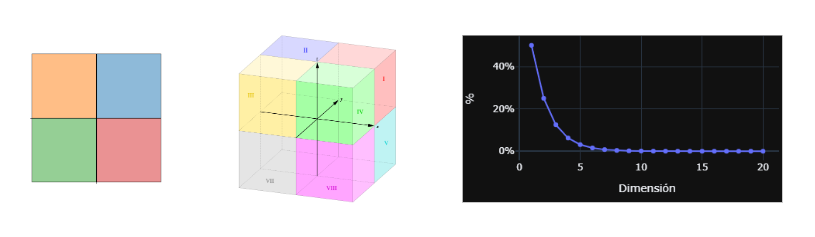
\includegraphics[width=\textwidth]{Figuras/maldicion_dimensionalidad.png}
    \caption[maldicion de la dimensionalidad]{Dimensionalidad y región dominada.}
    \label{fig:maldicion_dim}
\end{figure}

Una manera de resolver este problema es reducir la dimensión del espacio objetivo de los problemas estudiados, este enfoque se puede seguir usando escalarizaciones o definiendo cantidades útiles, esto último es lo que pretenden hacer los indicadores de calidad que definiremos en esta sección. Como mencionamos en la Sección \ref{sec:QIs}, los indicadores de calidad son propiedades de los conjuntos de soluciones que resumen sus características en valores que expresan, por ejemplo, qué tan separados están los individuos, cuántos individuos hay, qué tanto rango abarcan, qué tan cerca están de converger a un conjunto de referencia, qué tan uniformemente están separados, etc. Los indicadores no se usan explícitamente para reducir las dimensiones del problema; es decir, encontrando el frente de Pareto en el espacio de los indicadores, sino que se usa esta información a mayor nivel de la aproximación para tomar decisiones acerca de, por ejemplo, que solución mantener en caso de un empate. Los Indicadores de calidad también son importantes para comparar algoritmos, ya que, como veremos a continuación, es difícil saber cuándo una aproximación al frente de Pareto es mejor a otra. 

\subsection*{SMS-EMOA} \label{sec:SMS-EMOA}

Habiendo definido los indicadores y los algoritmos previos, en esta sección describiremos uno de los primeros IB-EMOAs llamado S Metric Selection-EMOA (SMS-EMOA) \cite{SMS-EMOA}. Este algoritmo es muy parecido a aquel de NSGA-II, que revisamos en la Sección \ref{sec:nsga2}, ya que también es no-elitista y usa non-dominated sorting. Sin embargo, en vez de usar el estimador de densidad basado en crowding distance utiliza un indicador de hipervolumen, además de esto es un algoritmo que cae en una familia de AE conocidos como steady-state. Esto significa que solamente se genera un hijo en cada una de las evaluaciones de la función de selección; es decir, es un algoritmo $\mu+1$. Se realiza de esta manera ya que, al usar el HV, se tiene que encontrar el individuo que menos contribuye en su maximización de toda la población de tamaño $N$. Así, se usa la Ecuación \eqref{eq:Contribucion} para iterar sobre los individuos y escoger el que se eliminará en la siguiente generación. Si se quedaran dos individuos nuevos, entonces habría que hacer $\binom{N}{2}=\frac{N(N-1)}{2}=O(N^2)$ comparaciones de modo que el algoritmo se volvería muy costoso. En el Algoritmo \ref{alg:SMS-EMOA} podemos ver el pseudocódigo de SMS-EMOA.

\begin{algorithm}
    \caption{SMS-EMOA}\label{alg:SMS-EMOA}
    \begin{algorithmic}[1] % The number indicates line numbering step
        \State $P_0$ = init;
        \State $t_0$ = init;

        \Repeat
        
        $q_{t+1}$ = genera($P_t$)
        
        $\{\mathcal{R}_1,\ldots,\mathcal{R}_v\}$ =fast-nds($P_t \cup \{q_{t+1}\})$
        
        $r=\text{argmin}_{S\in \mathcal{R}_v}\left( \text{HV}(s,\mathcal{R_v}) \right)$
        
        $P_{t+1}= Q \setminus \{r\}$;
        
        $t=t+1$;
        
        \Until condicion de termino

    \end{algorithmic}
\end{algorithm}

Este algoritmo es bueno en tareas que NSGA-II no lo era, como aumentando el número de objetivos hasta 4. El cálculo del HV para dimensiones mayores se vuelve costoso computacionalmente y, como se mencionó anteriormente, el cálculo es dependiente de la elección del punto de referencia. Esto puede afectar la diversidad y convergencia de las soluciones obtenidas.

Se han hecho muchos IB-EMOAs que, al igual que SMS-EMOA sólo utilizan uno de ellos para guiar su exploración y explotación del espacio de estados. Por lo tanto, heredan las virtudes y los defectos de depender tanto de una cualidad del conjunto de soluciones que se va generando, o del conjunto de referencia del frente de Pareto. Por ejemplo, los basados en HV generan muchas soluciones alrededor de la \emph{rodilla} y las fronteras del frente de Pareto, mientras que producen soluciones bien distribuidas para frentes convexos y lineales, además de tener buen desempeño en frentes degenerados \cite{HV_reference}, \cite{SMS-EMOA}. Los que están basados en R2, visto en la Sección \ref{sec:R2}, tienen buena distribución en frentes cóncavos, pero no hacen lo mismo para frentes convexos, degenerados o desconectados, dado a que los vectores de peso convexos intersectan esas geometría \cite{performance_pareto_front}, \cite{R2-EMOA}. Por esta razón, una extensión natural a los IB-EMOAs de un indicador, es usar varios indicadores para que sus objetivos estén en contraste, que puedan evitar problemas de sobre-especialización y que no sean dependientes de la forma del frente de Pareto.  

\section{PFI-EMOA} \label{sec:PFI-EMOA}

En esta sección se detalla el algoritmo usado en este trabajo. Recibe el nombre de Pareto Front Invariant EMOA (PFI-EMOA) y nace de la necesidad de encontrar un algoritmo que funcione para muchas dimensiones y a la vez que no tenga las restricciones mencionadas en el último párrafo de la sección anterior. La idea principal de este algoritmo es seguir con el marco principal de SMS-EMOA; es decir, usar non-dominated sorting para rankear las soluciones y usar un algoritmo steady-state para no hacer muchas comparaciones de contribuciones a indicadores. La diferencia principal es que se reemplaza el estimador de densidad de Hipervolumen que estaba presente en SMS-EMOA por una combinación de dos indicadores: IGD+ \eqref{eq:IGDp} y la Energía-S de Riesz \eqref{eq:S_energy}. Al ser estos dos indicadores de categorías diferentes (convergencia principalmente y diversidad) tendrán objetivos conflictuantes que obligarán a explorar una región distinta del espacio de estados. Estos dos indicadores se combinan por medio de la función aumentada de Tchebycheff,  qeue para un vector $\vec{x}=(x_0,x_1)$ está dada por


\begin{equation} \label{eq:ATCH}
    \text{ATCH}_{\vec{w}}(x_0,x_1)=\max_{i=0,1} \{w_ix_i\}+\alpha (x_0+x_1),  
\end{equation}


Sustituyendo cada uno de los indicadores tenemos
\begin{align*}
    \text{ATCH}_{\vec{w}}=({\text{IGD}}^+(A,Z),E_s(A)), \nonumber
\end{align*}

% \begin{align} \label{eq:ATCH}
%     \text{ATCH}_{\vec{w}}({\text{IGD}}^+(A,Z),E_s(A))=&\max \{w_0{\text{IGD}}^+(A,Z),w_1E_s(A)\}\\&+\alpha ({\text{IGD}}^+(A,Z)+E_s(A))
% \end{align}

donde $Z$ es un conjunto de referencia y $A$ es la aproximación al frente de Pareto.

Una característica interesante de hacer esta combinación es que se obtiene un indicador que no es consistente de Pareto. Esto se debe a un teorema probado en \cite{falcon-cardonaConstructionParetoCompliantCombined2022} que asegura que si se combina un indicador débilmente consistente de Pareto (IGD+) \eqref{eq:consistente_debil_Pareto} con uno que no lo es (Energía-S), entonces se tendrá como resultado uno que no es consistente de Pareto. Entonces se deben analizar los tres casos de la Figura \ref{fig:casos} como si fuera un problema de dominancia usual en dos dimensiones.

\begin{figure}[H]
    \centering
    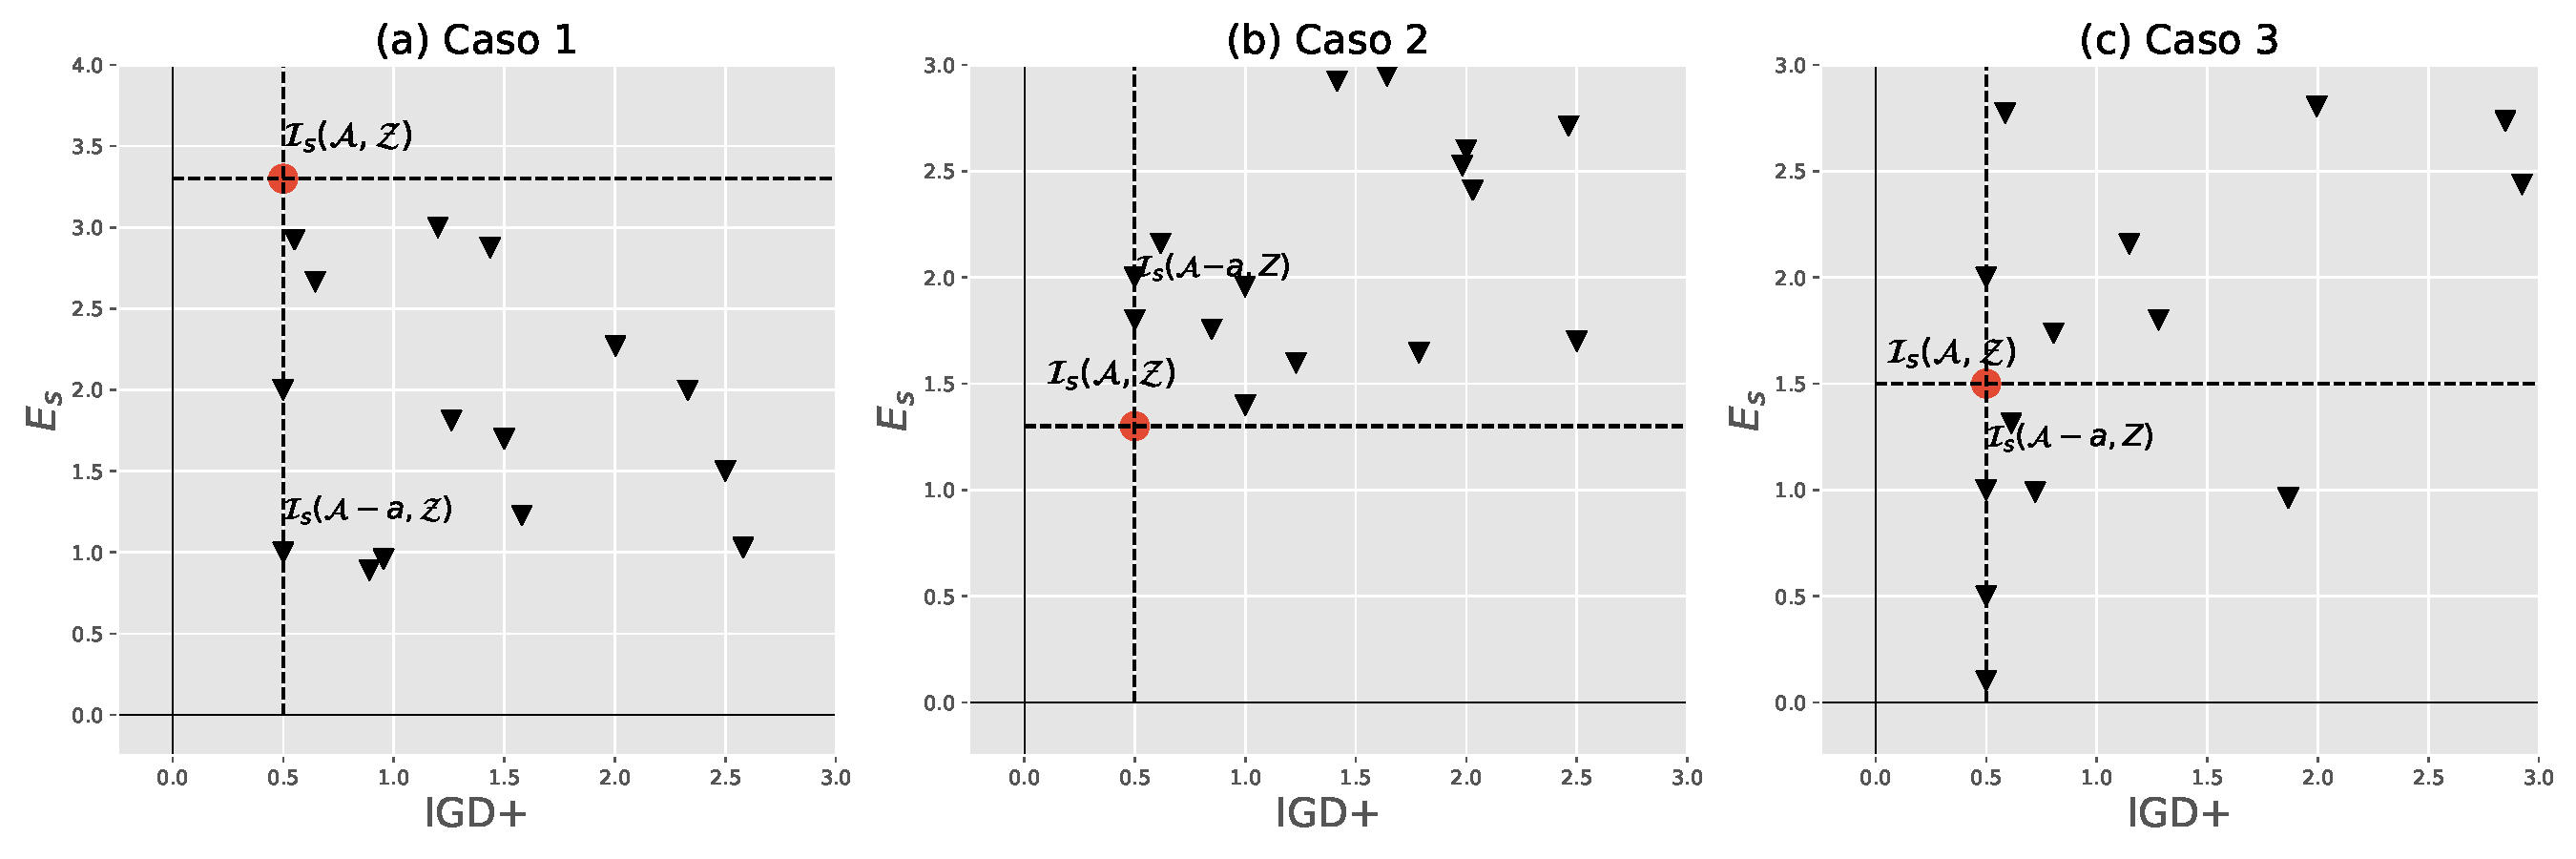
\includegraphics[width=\textwidth]{Figuras/casos.pdf}
    \caption[Tres casos para PFI.emoa]{Tres casos de selección diferentes dependiendo del comportamiento de la contribución al indicador combinado \eqref{eq:Contribucion}.}
    \label{fig:casos}
\end{figure}


En el caso 1, cada que una solución se remueve de $A$, $E_s$ se vuelve mejor. Entonces $\vec{I}_s(A,Z)$ está mutuamente no dominado contra las contribuciones de cada solución, $\vec{I}_s(A \setminus {\vec{a}},Z)$. Entonces $\text{ATCH}$ podría ser menor, igual o mayor antes y después de quitar la solución $\vec{a}$. En el caso 2, todos los vectores  $\vec{I}_s(A \setminus {\vec{a}},Z)$ están dominados por  $\vec{I}_s(A ,Z)$ por tener $E_s$ mayor, dado que $\text{ATCH}$ preserva orden\footnote{Esto quiere decir que $\text{ATCH}(\vec{I}_s(A,Z))< \text{ATCH}(\vec{I}_s(A \setminus {\vec{a}},Z))$}. Finalmente el caso 3 es una combinación de ambos. Como existe una solución que no contribuye a la convergencia del algoritmo, en cualquiera de estos 3 casos, se elimina la solución que peor contribuya a la Energía-S. En el Algoritmo \ref{alg:PFI-EMOA} podemos ver el pseudocódigo de PFI-EMOA.


\begin{algorithm}
    \caption{PFI-EMOA}\label{alg:PFI-EMOA}
    \begin{algorithmic}[1] % The number indicates line numbering step
        \Require Vector de pesos $\vec{w}\in \mathbb{R}^2$ 
        \Ensure  Aproximación del Frente de Pareto
        \State $P_0$ = init;

        \Repeat
                
        $q_{t+1}$ = genera($P_t$)
        
        $\{\mathcal{R_1},\ldots,\mathcal{R}_k\}$ =fast-nds($P_t \cup \{q_{t+1}\})$
        
        \If{$|R_k|>1$}  

        \State $z_i^{\max} = \max_{\vec{a}\in Q} a_i, i=1,\ldots,m$
        \State $z_i^{\min} = \min_{\vec{a}\in Q} a_i, i=1,\ldots,m$

        Normalizar $\{R_j\}_{j=1,\ldots,k}$ usando $\vec{z}^{\max}, \vec{z}^{\min}$

        \State $B = \{\vec{b} \ |\  \text{IGD}^+(\mathcal{R}_k \setminus \{\vec{b}\})=\text{IGD}^+(\mathcal{R}_k,\mathcal{R}_1), \forall \vec{b} \in \mathcal{R}_k\}$
        \If{$|B|>0$}
        $\vec{a}_{\text{worst}}=\text{argmax}_{\vec{b}\in B} C_{E_s}(\vec{b},\mathcal{R}_k)$ 
        \Else 
        
        $\vec{a}_{\text{worst}}=\text{argmax}_{\vec{r}\in \mathcal{R}_k} \text{ATCH}_{\vec{w}}(\vec{I}_s(\mathcal{R}_k \setminus \{r\}),\mathcal{R}_1)$ 
        
        

        \EndIf

            \Else 

            $\vec{a}_{\text{worst}}$ es la única solución de $\mathcal{R}_k$
        \EndIf 

        $P=Q\setminus \{\vec{a}_{\text{worst}}\}$
     
        
        \Until condicion de termino

    \end{algorithmic}
\end{algorithm}

Iremos explicando este algoritmo línea por línea. Al inicio se requiere como parte de la entrada un vector de pesos. Esto será importante ya que en \cite{PFI} sólo se usó una combinación fija de pesos para una serie de problemas prueba (revisaremos estos problemas en el próximo capítulo). Enseguida, ya entrando en el algoritmo se inicializa la población en la línea 1 y se comienza un ciclo en la línea 2 hasta cumplir la condición de término . En este trabajo la condición de paro se estableció como las iteraciones necesarias para superar un número fijo de generaciones. Las siguientes dos líneas sin número abajo de \textbf{repeat} generan un hijo a través de operadores evolutivos y abajo se utiliza non-dominated sorting para rankear las soluciones, como en la Figura \ref{fig:nsga1}, siendo $\mathcal{R}_k$ las soluciones de la peor capa. 
Siguiendo con la línea 3, entramos al \textbf{if} que nos pregunta si existe más de una solución en la última capa, si la hay, entonces hay que usar el estimador de densidad que se desglosa en varios casos. Primero, en las líneas 4 y 5 se normaliza el rango de los objetivos dividiendo entre el máximo y el mínimo de cada dimensión. Después, en la línea 6 se construyen los diferentes casos que corresponden a la Figura \ref{fig:casos}. Primero, vemos el conjunto de soluciones que no contribuyen al indicador de $\text{IGD}^+$, si tiene más de una solución, se elimina aquella con peor contribución a la Energía-S de Riesz. En caso contrario se usa el estimador de densidad dado por la función aumentada de Tchebycheff \eqref{eq:ATCH}. Finalmente, vemos el caso donde la última capa sólo tuvo un elemento, entonces no hay que escoger cuál eliminar porque solo hay un candidato. En la penúltima línea se actualiza la población quitando la peor solución $\vec{a}_{\text{worst}}$ y se revisa si se alcanzó la condición de término para regresar la aproximación al frente de Pareto. 

\section{Pruebas Estadísticas y Comparación de algoritmos} \label{sec:pruebas_estadisticas}

El interés principal de este trabajo es el de comparar el desempeño de distintas configuraciones de pesos en el algoritmo \ref{sec:PFI-EMOA}. Para fines prácticos, esto se puede entender como comparar el desempeño de algoritmos distintos. Así, planteareamos de manera general cómo se pueden comparar un conjunto de algoritmos que dan un resultado distinto para las mismas entradas\footnote{Estas entradas corresponden a las poblaciones iniciales y pueden ser comparadas entre sí porque se generan usando semillas aleatorias.}. Dado que los EMOAs tienen un comportamiento estocástico, tendremos que hacer muchas corridas de los algoritmos y comparar poblaciones de resultados entre sí. Es por ello que recurriremos a pruebas estadísticas para determinar si el desempeño de los algoritmos fue distinto. La manera en la que decidiremos si un algoritmo tuvo mejor desempeño que otro es usando nuevamente los inidcadores de calidad, pero ahora calculandolos sobre la población final (recordando que la salida de los EMOAs son conjuntos de aproximación al frente de Pareto).

Entonces, por cada población final, haremos el cálculo de cada uno de los indicadores que están en \ref{sec:AE} para cada corrida de cada algoritmo y los compararemos usando las pruebas estadísticas que se exponen en esta sección. Al ser muchos los indicadores donde haremos las pruebas, tendremos muchos resultados acerca de qué solución conviene dependiendo de la característica que busquemos de la solución. Es decir, tendremos resultados del tipo: \emph{El algoritmo PFI-EMOA con una confifuración de pesos $\vec{w}_1$ obtiene, de manera estadísticamente significativa, un Hipervolumen mayor al algoritmo PFI-EMOA con pesos $\vec{w}_2$ para el problema  prueba específico con $n$ objetivos}.   

En estos problemas, la distribución que siguen los valores de los indicadores no es conocida ya que el fenómeno es suficientemente complejo como para rastrearlo de esta manera. Así, para realizar la comparación del desempeño de los algoritmos en los diferentes indicadores tendremos que hacer uso de pruebas no paramétricas que comparen nuestras muestras. En particular usaremos la prueba de Friedman, que nos ayudará a decidir si existe una diferencia entre poblaciones. Es decir, probaremos si hay o no evidencia para rechazar la siguiente hipótesis nula: \emph{Al menos una de las muestras viene de una distribución distinta a las demás}. 

Además, usaremos la prueba de Wilcoxon, en la Sección \ref{sec:Wilcoxon}, para comparar uno a uno las diferentes configuraciones de los algoritmos y así poder distinguir qué distribuciones tienen mediana superior (o inferior, según si se quiere maximizar o minimizar el indicador) a las demás. De esta manera podremos decir que hay evidencia para rechazar la hipótesis nula de que una distribución no tiene mediana superior o inferior a la otra.

En esta sección se detallan las pruebas que usaremos más adelante para comparar el desempeño de algoritmos en una misma tarea. Ambas pruebas son no paramétricas ya que desconocemos la distribución del desempeño del algoritmo dados los parámetros que pondremos. Las dos pruebas que veremos en esta sección tienen su implementación en la librería de Python de  \href{https://docs.scipy.org/doc/scipy/reference/stats.html}{scipy.stats} que usaremos en el capítulo de resultados. 

Cabe destacar que ambas pruebas tienen modificaciones cuando se toman en cuenta empates entre las diferentes poblaciones. Sin embargo, como estamos considerando una variable aleatoria continua (el valor de indicadores de los conjuntos de aproximación) la probabilidad de coincidencias es cero así que presentamos las pruebas sin esta consideración.


\subsection{Prueba de Friedman} \label{sec:Friedman}

La prueba de Friedman \cite{hollanderNonparametricStatisticalMethods2015} es una prueba no paramétrica utilizada para detectar diferencias en tratamientos a través de múltiples bloques que están \textbf{relacionados entre sí}. Es una alternativa a la ANOVA de medidas repetidas cuando no se cumplen las suposiciones de normalidad. Se usa principalmente en diseños de poblaciones iniciales aleatorizados donde las observaciones dentro de cada bloque (o sujetos) son \textbf{dependientes}. En el contexto de este trabajo, podemos pensar en los sujetos que están relacionados como las poblaciones iniciales con las que comienza su búsqueda cada algoritmo con diferentes parámetros. Dichas inicializaciones están controladas por diferentes semillas de modo que podemos decir que están relacionadas. Por otro lado, los tratamientos que suelen formar parte de esta prueba tendrían su análogo en este trabajo en la salida de cada algoritmo; es decir, el cálculo de un indicador de calidad aplicado al conjunto de aproximación final.  

Así, la prueba de Friedman asume que tenemos \( k \) algoritmos aplicados a \( n \) poblaciones iniciales. La hipótesis nula \( H_0 \) establece que las medianas de los indicadores calculados de la salida de los algoritmos son iguales, mientras que la hipótesis alternativa \( H_1 \) indica que al menos una de ellas es diferente.

Los supuestos de la prueba de Friedman son los siguientes:
\begin{itemize}
    \item Los datos consisten en \( n \) poblaciones iniciales, cada uno con \( k \) algoritmos distintos aplicados sobre ellas.
    \item Las observaciones son ordinales o continuas.
\end{itemize}

Para realizar la prueba, los pasos son los siguientes:

\begin{enumerate}
    \item Asignar rangos dentro de cada población inicial. Para cada población inicial \( j \) y salida del algoritmo \( i \), se ordenan las observaciones y se les asigna un rango \( R_{ij} \).
    \item Calcular la suma de rangos para cada salida del algoritmo \( i \):
    \[
        R_i = \sum_{j=1}^{n} R_{ij}
        \]
\item Calcular el estadístico de prueba \( Q \), que se define como:
        \[
            Q = \frac{12}{nk(k+1)} \sum_{i=1}^{k} \left( R_i - \frac{n(k+1)}{2} \right)^2
            \]
            donde \( n \) es el número de poblaciones iniciales y \( k \) es el número de algoritmos.
        \end{enumerate}

El estadístico \( Q \) sigue una distribución \( \chi^2 \) con \( k-1 \) grados de libertad bajo la hipótesis nula. La fórmula de \( Q \) se puede expresar de manera más simplificada como:
   \[
   Q = \frac{12}{nk(k+1)} \left[ \sum_{i=1}^{k} R_i^2 - \frac{nk(k+1)^2}{4} \right]
   \]

% \begin{figure}[H]
%     \centering
%     \includegraphics[width=\textwidth]{Figuras/friedman.pdf}
%     \caption[Prueba de Friedman]{Ilustración de la prueba de Friedman.}
%     \label{fig:friedman}
% \end{figure}



% \subsection{Kruskal-Wallis} \label{sec:Kruskal-Wallis}

% La prueba de Kruskal-Wallis \cite{Kruskal} es una extensión no paramétrica de la ANOVA \cite{geisserStatisticalPrinciplesExperimental1963} de un solo factor. Se utiliza cuando hay tres o más poblaciones independientes \footnote{Para dos poblaciones recibe el nombre de Mann-Whitney U.} de datos de los que nos interesa saber si provienen de la misma distribución, especialmente cuando las suposiciones de normalidad y homocedasticidad (requeridas por ANOVA) no se cumplen. En la Figura \ref{fig:kruskal} se simularon poblacionales distintas para obtener diferentes resultados en las pruebas de ANOVA y Kruskal. Cada una de las distribuciones mostradas es:
% \begin{enumerate}
%     \item Las tres poblaciones se generan de tres normales con medias $\mu_1=50, \mu_2=51, \mu_3=52$ y la misma desviación estándar $\sigma_1=\sigma_2=\sigma_3=10$.
%     \item Se generan dos normales $X_1\sim N(50,10), X_2\sim N(50,20)$ y una exponencial con la misma media $X_3\sim \text{Exp}(\lambda=50)$.
%     \item Se establece un valor de mediana, aunque la media varía caso a caso. Así, tenemos $X_1\sim N(10,1)$, $X_2 \sim \text{Exp}(10/\log 2)$, mientras que $X_3$ es una distribución bimodal que viene de dos normales cada una centrada a una distancia de 5 de la mediana establecida.
%     \item Aquí todas las distribuciones son diferentes, tanto las medias como las medianas; $X_1\sim N(50,10), X_2\sim N(70,10), X_3\sim N(90,10)$.
% \end{enumerate}

% Así, logramos tener 4 casos diferentes dependiendo si se rechaza o acepta la hipótesis nula de Kruskal-Wallis o ANOVA. Explicaremos más adelante por qué sucede cada caso de la Figura \ref{fig:kruskal}.

% \begin{figure}[H]
%     \centering
%     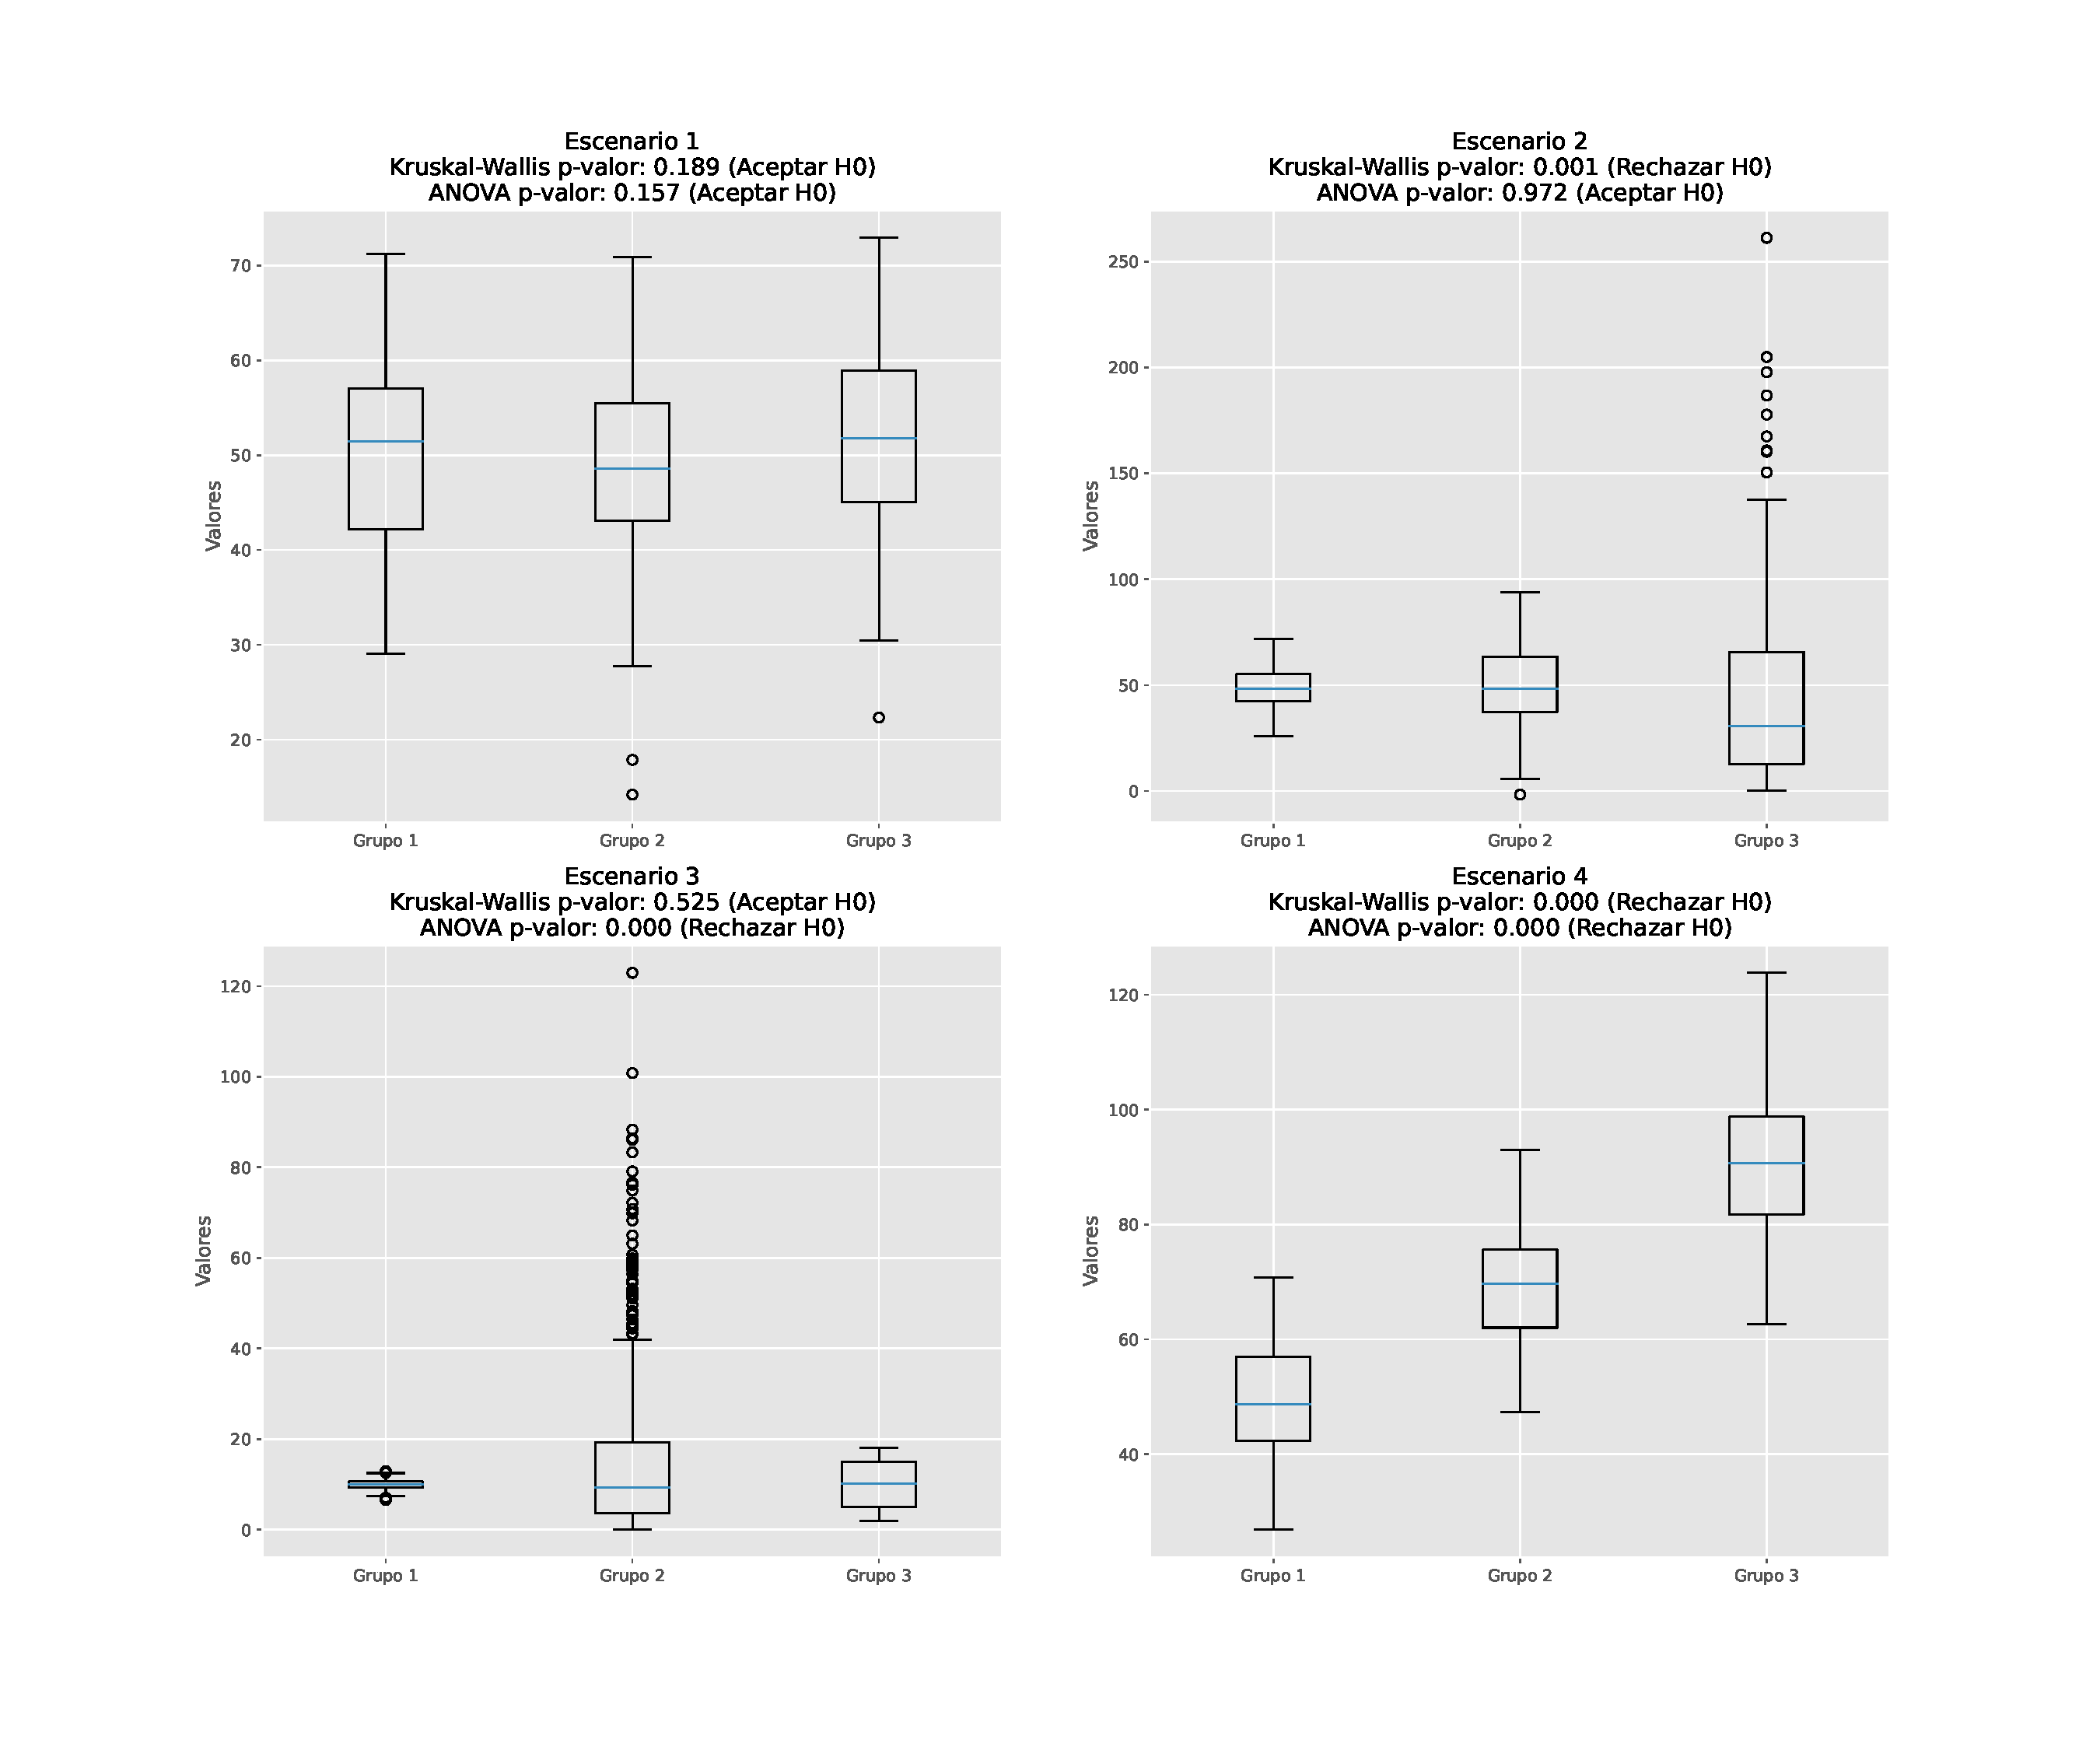
\includegraphics[width=\textwidth]{Figuras/kruskal.pdf}
%     \caption[Prueba de Kruskal]{Ilustración de la prueba de Kruskal.}
%     \label{fig:kruskal}
% \end{figure}


% En Kruskal-Wallis la hipótesis nula \( H_0 \) es que las medianas de todas las poblaciones son iguales mientras que la hipótesis alternativa \( H_1 \) es que al menos existe una de ellas donde la mediana es distinta. Las poblaciones no necesariamente tienen que tener el mismo número de elementos.

% Los supuestos de la prueba son los siguientes:
% \begin{itemize}
%     \item La variable de respuesta es ordinal o continua. Es decir existe una cantidad mejor a otra.
%     \item Independencia. Las observaciones de cada grupo son independientes entre sí.
%     \item Distribuciones tienen formas similares: Aunque no pedimos que sean normales, para comparar los rangos necesitamos que sean distribuciones similares con, tal vez, diferentes parámetros.
% \end{itemize} 

% Para construir el estadístico de prueba primero se hace un ranking de todos los elementos en todos los diferentes poblaciones, es decir, se ordenan todos los elementos de menor a mayor y se le asigna su posición en el ordenamiento a cada uno de ellos, a esta cantidad se le llama el rango del individuo $i$ \footnote{En este desarrollo se presenta la deducción para el caso donde no hay empates. }. 

% Después se calcula el rango promedio global, que se denota como \( \bar{R} \), mediante:

% $$
% \bar{R} = \frac{\sum_{i=1}^{g} R_i}{N} = \frac{1 + 2 + \ldots + N}{N} = \frac{N(N + 1)/2}{N} = \frac{N + 1}{2}.
% $$


% donde 
% \begin{itemize} 
%     \item \( g \) es el número de poblaciones o grupos.
%     \item \( n_i \) es el número de observaciones en la población \( i \).
%    \item \( N =\sum_{i=1}^n n_i\) es el número total de observaciones.
%    \item \( R_i =\sum_{j=1}^{n_i} R_{ij}\) es la suma de los rangos en la población $i$-ésima.
% \end{itemize}



% De la misma forma se define el rango promedio para cada población \(j\), \( \bar{R_j} \), se calcula como:

% $$
% \bar{R_j} = \frac{R_j}{n_j}.
% $$

% Ahora se calcula el cuadrado de la diferencia entre los rangos promedio con rango promedio global para cada población, ponderada por el tamaño de la misma, obteniendo:

% $$
% n_i (\bar{R_i} - \bar{R})^2 = n_i \left(\frac{R_i}{n_i} - \frac{N + 1}{2}\right)^2 = \frac{R_i^2}{n_i} - N (N+1) + \frac{n_i (N + 1)^2}{4}.
% $$

% Se suman todas estas diferencias para obtener:

% $$
% \sum_{i=1}^{g} \frac{R_i^2}{n_i} - g N (N + 1) + (N + 1)^2 \sum_{i=1}^{g} \frac{n_i}{4}.
% $$

% Así tenemos una cantidad que se comporta como una $\Xi$ cuadrada salvo un factor de normalización \( \frac{12}{N (N + 1)} \) para obtener \( H \) el estadístico de prueba:

% $$
% H = \frac{12}{N(N + 1)} \left(\sum_{i=1}^{g} \frac{R_i^2}{n_i} - N (N + 1)\right) + 3(N + 1).
% $$

% Y simplificando, se obtiene la Ecuación \ref{eq:Kruskal-Wallis} para $H$:

% \begin{equation} \label{eq:Kruskal-Wallis}
% H = \frac{12}{N(N + 1)} \sum_{i=1}^{g} \frac{R_i^2}{n_i} - 3(N + 1),
% \end{equation}

    
% La  \( H \) se distribuye como una distribución \( \chi^2 \) con \( g-1 \) grados de libertad. De esta forma podemos probar la hipótesis nula a una significancia de $\alpha$, rechazando si el $p$-valor es menor a $\alpha$ y aceptando si es mayor. 

% Podemos entender la Figura \ref{fig:kruskal} viendo que las distribuciones de los datos simulados se escogieron de modo que tuvieramos control sobre la media y la mediana de cada distribución. A ANOVA le importa la similitud entre las medias y a Kruskal-Wallis le importan los rangos. Entonces, al tomar una distribución con medias iguales y medianas diferentes obtenemos la subfigura superior derecha. Cambiando ahora la media, pero dejando la mediana igual (las lineas del boxplot están niveladas), tenemos que rechazamos ahora ANOVA (las medias son diferentes), pero aceptamos que las medianas son iguales y por lo tanto aceptamos $H_0$ para Kruskal-Wallis.

Ya teniendo el estadístico de prueba podemos comparar su probabilidad de ocurrencia bajo la hipótesis nula de acuerdo a un nivel de significancia prestablecido. 

\subsection{Prueba de Wilcoxon} \label{sec:Wilcoxon}

La prueba de Wilcoxon Signed-Rank \cite{Wilcoxon} es una prueba estadística no paramétrica que se utiliza para comparar dos muestras pareadas como vemos en la Figura \ref{fig:Wilcoxon}. Es una alternativa no paramétrica a la prueba $t$ de student \cite{geisserStatisticalPrinciplesExperimental1963} \textbf{para muestras pareadas} y es útil cuando no se pueden asumir distribuciones normales en la diferencia de las observaciones. 

\begin{figure}[H]
    \centering
    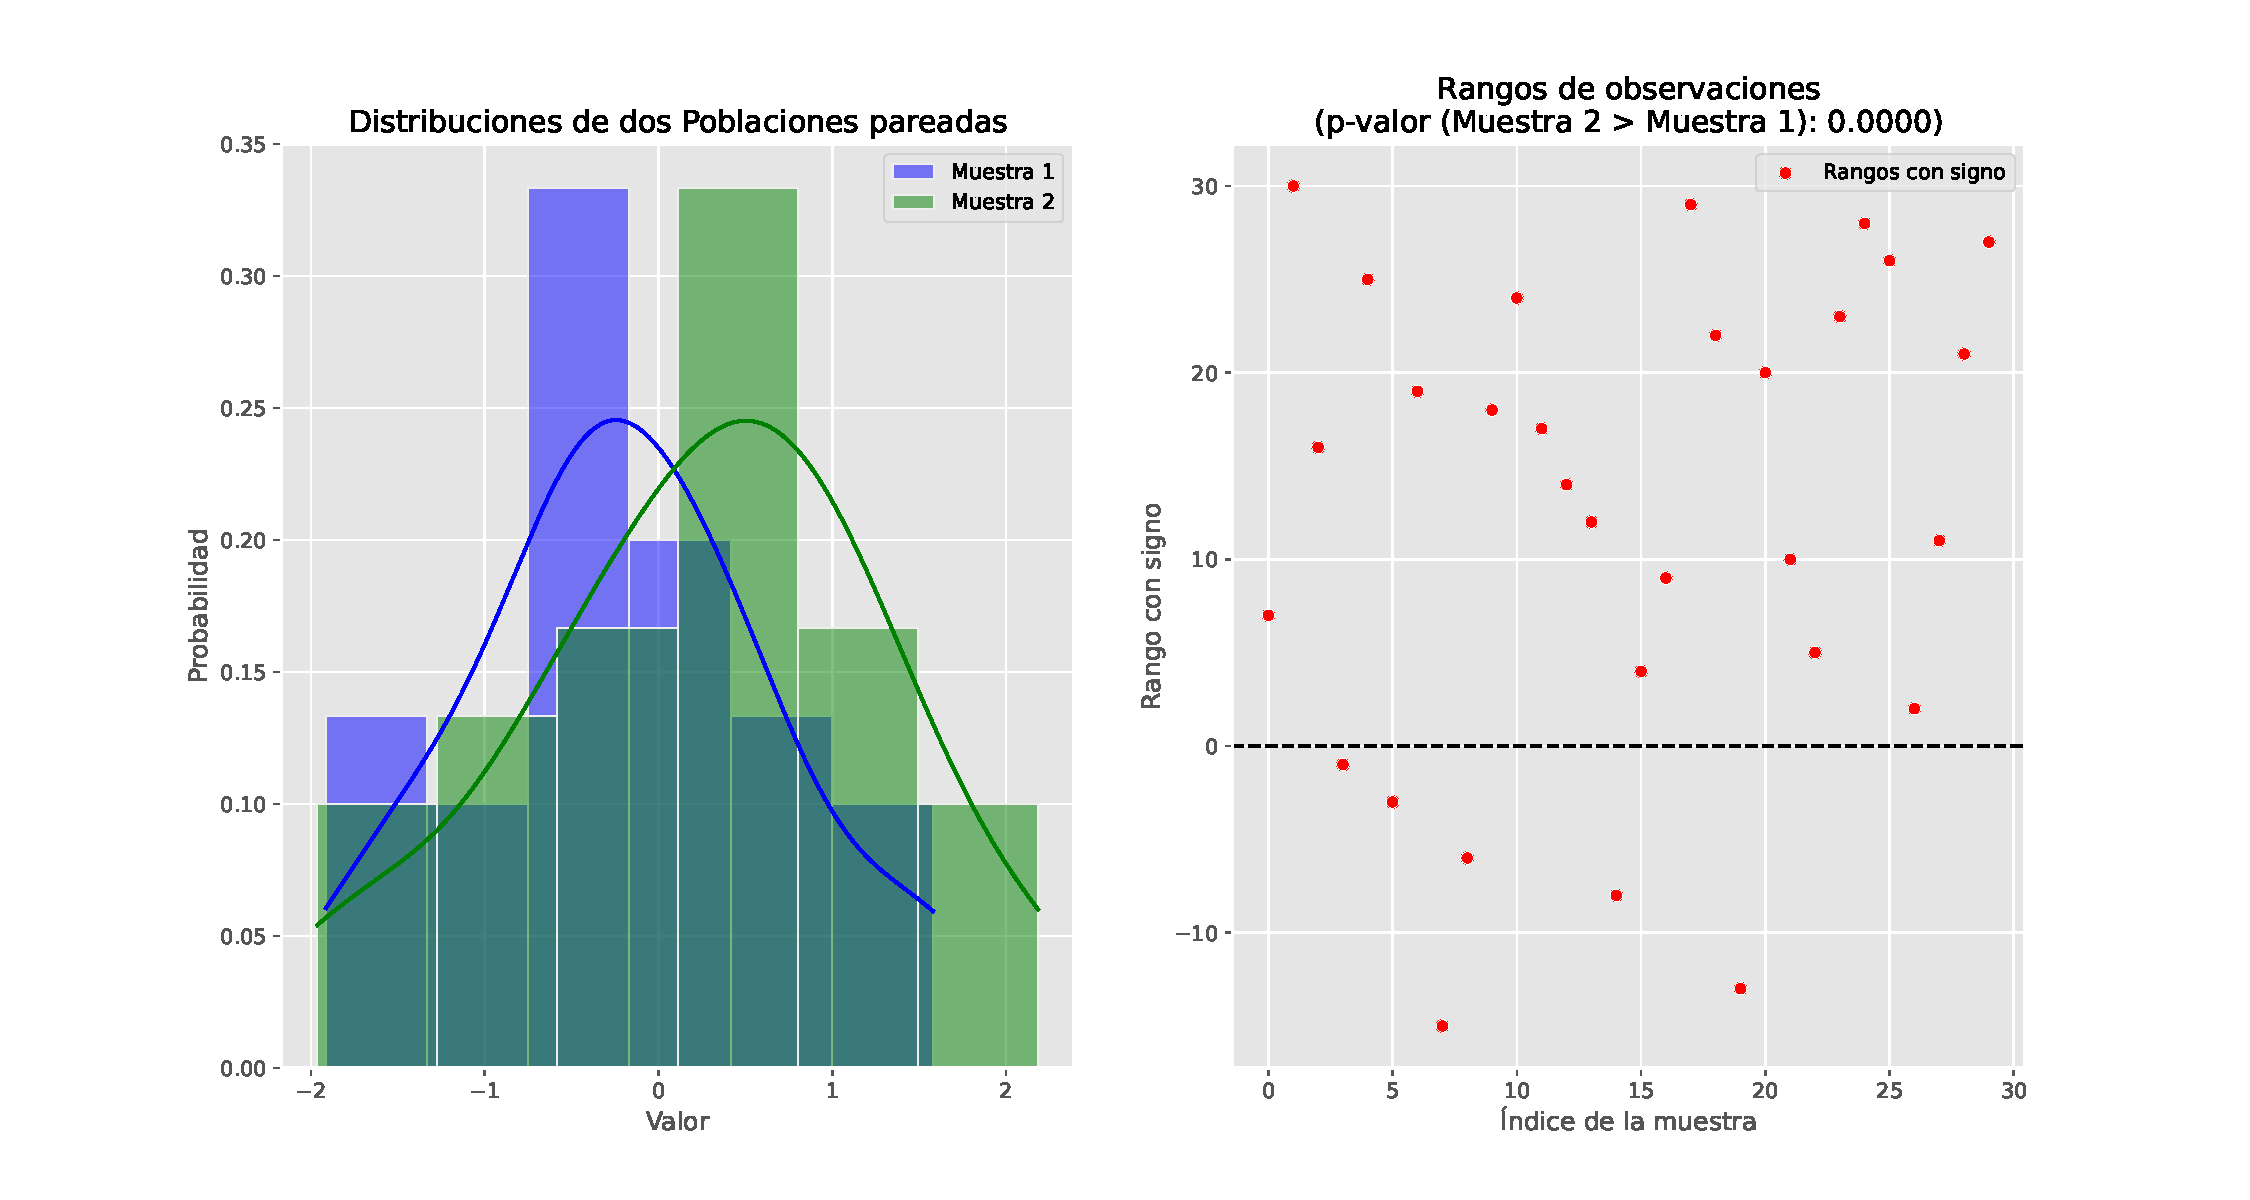
\includegraphics[width=\textwidth]{Figuras/Wilcoxon_vis.pdf}
    \caption{Visualización de lo que hace la prueba de Wilcoxon.}
    \label{fig:Wilcoxon}
\end{figure}


En el capítulo 4 realizaremos esta prueba para comparar algoritmos evolutivos multiobjetivo que tienen diferentes parámetros. Así, la discusión de esta prueba se da en términos de este caso particular.

Supongamos que tenemos un conjunto de $n$ entradas diferentes, que llamaremos poblaciones y denotaremos $P_i, i\in\{1,2,\ldots,n\}$. Estas poblaciones se inicializan de manera aleatoria, pero para cada $i$ se hace con una semilla diferente. Las poblaciones iniciales se mapean a un número real usando dos algoritmos distintos, $A_1,A_2$ \footnote{En nuestro caso las entradas son poblaciones de individuos que se evolucionan con ayuda de un EMOA. Los $A_1,A_2$ son el mismo algoritmo sólo que con diferentes hiperparámetros. Estos algoritmos tienen como salida una aproximación del frente de Pareto y el mapeo a los números reales $A_i(P_j)$ es un indicador de calidad que se obtiene de la aproximación al frente.} de modo que la salida del algoritmo son dos valores reales por cada población $A_1(P_i), A_2(P_i)$. Estos últimos resultados son dependientes porque comenzaron con la misma población, de modo que los consideramos observaciones pareadas. De este modo, obtenemos las diferencias de cada par de observaciones para obtener la Tabla \ref{tab:datos_pareados}.

\begin{table}[H]
    \centering
    \begin{tabular}{|c|c|c|c|}
    \textbf{Población Inicial $P_i$} & \textbf{Algoritmo 1} & \textbf{Algoritmo 2} & \textbf{Diferencias}    \\ \hline
    $P_1$                            & $A_1(P_1)$           & $A_2(P_1)$           & $Z_1=A_1(P_1)-A_2(P_1)$ \\
    $P_2$                            & $A_1(P_2)$           & $A_2(P_2)$           & $Z_2=A_1(P_2)-A_2(P_2)$ \\
    $\vdots$                         & $\vdots$             & $\vdots$             & $\vdots$                \\
    $P_n$                            & $A_1(P_n)$           & $A_2(P_n)$           & $Z_n=A_1(P_n)-A_2(P_n)$
    \end{tabular}
\caption[Algoritmos a comparar]{Vemos la estructura de los algoritmos a comparar.}
\label{tab:datos_pareados}
\end{table}


Las suposiciones de la prueba de Wilcoxon \cite{hollanderNonparametricStatisticalMethods2015} son parecidas a aquellas de la de Friedman:

\begin{itemize}
    \item Las observaciones pareadas tienen un carácter ordinal o real y los $Z_i$ son mutuamente independientes. 
    \item Cada $Z$ viene de una distribución continua que es simétrica alrededor de una mediana común $\theta$, llamada el efecto del tratamiento.
    %  Si $F_i$ es la función de probabilidad de $Z_i$, tenemos que 
    % $$ F_i(\theta+t)+F_i(\theta -t)=1, \,\, \forall t, i .$$
\end{itemize}

Ya con estas definiciones la hipótesis nula se puede formular como $$ H_0: \theta=0 $$
Es decir, cada una de las distribuciones (no necesariamente iguales entre cada $Z_i$)  de las diferencias entre un algoritmo y otro está distribuida simétricamente alrededor del 0. 

Para realizar la prueba hacemos lo siguiente 

\begin{itemize}
    \item Para cada par de observaciones pareadas \(i\), se calcula la diferencia \(d_i = x_i - y_i\).
    \item Se ordenan las diferencias absolutas \(|d_i|\) y se les asigna (al igual que en Friedman) rangos \(R_i\) desde el más pequeño al más grande. 
    \item Se separan las diferencias en dos grupos: diferencias positivas y diferencias negativas. Calculamos las sumas de los rangos para cada grupo  y las denotamos como \(W_+\) y \(W_-\) para las diferencias positivas y negativas respectivamente. Es decir, 
    \begin{align*}
    W_+= \sum_{d_i>0} \text{rank}(d_i) +\frac{1}{2}\sum_{d_i=0}\text{rank}(d_i), \nonumber\\
    W_-= \sum_{d_i<0} \text{rank}(d_i) +\frac{1}{2}\sum_{d_i=0}\text{rank}(d_i). \nonumber
    \end{align*}
\end{itemize}

El estadístico de prueba, está dado por el menor de \(W_+\) y \(W_-\), esto se debe a que estamos asumiendo que la distribución de las diferencias es la misma para cada una de ellas y es simétrica con respecto al origen ($\theta=0$). Entonces, la probabilidad de caer de un lado o del otro del cero sería de 1/2 y simplemente tenemos que ver cuál fue el número de casos que cayeron de un lado y ver la probabilidad de ocurrencia. Para dar un ejemplo concreto supongamos que tenemos $B$ casos donde la diferencia $Z$ es positiva. Después ordenamos estas diferencias para obtener los rangos\footnote{No hay menor o igual porque asumimos que las distribuciones son continuas, entonces la probabilidad de caer exactamente en el mismo punto es cero.} 

$$r_1 < r_2 <\cdots r_B.$$

Si tuvieramos, por ejemplo, 3 observaciones $Z_1,Z_2,Z_3$, la configuración de signos de estas observaciones nos da un total de 8 y bajo la $H_0$ cada uno de estos es igual de probable. Entonces tenemos $1/8$ de encontrar cada una de las configuraciones.

Lo que medimos con la prueba es la suma de rangos totales sí que supongamos que tenemos $T^+=3$, entonces basta contar las maneras de obtener este número para así obtener la probabilidad de que lo obtengamos dado que la hipotesis nula es cierta. De acuerdo a la Tabla \ref{tab:tmas}, tenemos que existen 2 formas de obtener $T^+=3$; cuando $r_1=3$ y cuando $r_1=1,r_2=2$, es decir, en el primer caso sólo existió una diferencia positiva $Z_i$ y fue la más pequeña de todas en valor absoluto, mientras que en el segundo hay dos diferencias positivas, las dos más grandes. Entonces vemos que la probabilidad de obtener $T^+=3$ esta dada por la suma de estos dos eventos y obtenemos $$ \mathbb{P}\left[ T^+=3 \right] =\frac{2}{8}.$$



\begin{table}[H]
    \centering
    \begin{tabular}{|c|c|c|c|}
    \textbf{B} & \textbf{$(r_1,\ldots,r_B)$} & \begin{tabular}[c]{@{}l@{}}Probabilidad de que\\ ocurra dado $H_0$\end{tabular} & $T^+=\sum_{i=1}^B r_i$ \\ \hline
    0          &                             & $\frac{1}{8}$                                  & 0                                                                                  \\
    1          & $r_1=1$                     & $\frac{1}{8}$                                  & 1                                                                                  \\
    1          & $r_1=2$                     & $\frac{1}{8}$                                  & 2                                                                                  \\
    1          & $r_1=3$                     & $\frac{1}{8}$                                  & 3                                                                                  \\
    2          & $r_1=1,r_2=2$               & $\frac{1}{8}$                                  & 3                                                                                  \\
    2          & $r_1=1, r_2=3$              & $\frac{1}{8}$                                  & 4                                                                                  \\
    2          & $r_1=2,r_2=3$               & $\frac{1}{8}$                                  & 5                                                                                  \\
    3          & $r_1=1,r_2=2,r_3=3$         & $\frac{1}{8}$                                  & 6                                                                                 
    \end{tabular}
\caption[Rankings y probabilidades]{Vemos todos los casos para los rankings de las diferencias positivas y su respectiva probabilidad.}
\label{tab:tmas}
\end{table}

Entonces se puede tomar como estadístico de prueba cualesquiera de las diferencias positivas y negativas y seguir el procedimiento de arriba. Para facilitar el cálculo de las combinaciones, se suele tomar el mínimo. Es decir, el estadístico para la prueba está dado por 

$$
T = \min(T_+, T_-).
$$


Para muestras grandes, la distribución de \(T\) se aproxima bien con una distribución normal y se puede convertir en una normal estándar con los siguientes factores

$$z= \frac{T-\frac{1}{4}N(N+1)}{\frac{1}{24}N(N+1)(2N+1)}.$$

Cuando se quiere hacer una prueba de un lado, es decir, si alguna de las poblaciones tiene mediana mayor o menor que otra, se toma solamente la parte positiva o negativa de las diferencias. Esto será útil en los siguientes capítulos cuando comparemos algoritmos ejecutados con diferentes configuraciones de parámetros. Una diferencia importante con respecto a la prueba $t$ es que, dado que la diferencia se convierte en rangos, no importa tanto la magnitud de la misma, sólo su orden relativo, de esta forma, la prueba de Wilcoxon no es tan sensible a outliers. 


\subsection{Análisis post-hoc y Family-wise Error Rate} \label{sec:FWER_Bonferroni}



En el análisis estadístico, cuando se realizan múltiples comparaciones o pruebas simultáneamente, incrementa la probabilidad de cometer errores de Tipo I (rechazar una hipótesis nula verdadera). Este fenómeno se conoce como la tasa de error familiar (FWER, por sus siglas en inglés: Family-wise Error Rate). La FWER es la probabilidad de cometer al menos un error de Tipo I entre todas las comparaciones.

Si se realizan $m$ pruebas estadísticas independientes, cada una con un nivel de significancia $\alpha$, la probabilidad de no cometer un error de Tipo I en una cada una de las prueba por sí misma es de $1 - \alpha$. Por lo tanto, la probabilidad de no cometer ningún error de Tipo I en las $m$ pruebas es $(1 - \alpha)^m$. Así, la probabilidad de cometer al menos un error de Tipo I es el complemento de este valor:

\begin{equation} \label{eq:FWER}
\text{FWER} = 1 - (1 - \alpha)^m.
\end{equation}

Al aumentar $m$, esta probabilidad crece, lo que incrementa el riesgo de falsas alarmas. Existen varios métodos para controlar la FWER, entre ellos se encuentra la corrección de Bonferroni.

La corrección de Bonferroni es una técnica que se considera conservadora y es usada  para ajustar los niveles de significancia y controlar el FWER. La idea básica es dividir el nivel de significancia $\alpha$ por el número total de pruebas $m$. Es decir, en lugar de utilizar $\alpha$ como el nivel de significancia para cada prueba individual, se utiliza $\alpha_{\text{Bonferroni}}$ definido como:

\begin{equation} \label{eq:Bonferroni}
\alpha_{\text{Bonferroni}} = \frac{\alpha}{m}.
\end{equation}

De esta manera, la probabilidad de cometer un error de Tipo I en cualquier prueba individual es reducida, y la probabilidad de cometer al menos un error de Tipo I en cualquiera de las $m$ pruebas se mantiene por debajo del nivel de significancia general $\alpha$.


\subsubsection{Limitaciones de las correcciones al FWER}

Es bastante debatido \cite{pernegerWhatWrongBonferroni1998}, \cite{nakagawaFarewellBonferroniProblems2004}, \cite{goemanMultipleHypothesisTesting2014}  cuando se debería de usar alguna corrección al FWER debido a que el error del que nos protege parece ser demasiado exigente. Las correcciones nos piden que ninguno de los rechazos de $H_0$ sea por probabilidad mayor a $\alpha$. Esto podría hacer que rechazáramos resultados interesantes sólo por el hecho de haber realizado análisis en conjunto. Esto quiere decir que puede llevar a un incremento en los errores de Tipo II (no rechazar una hipótesis nula falsa), reduciendo así el poder estadístico del análisis. Existen otras técnicas menos conservadoras, como la corrección de Holm-Bonferroni y la corrección de Sidak. De la misma forma de acuerdo a las dos pruebas expuestas anteriormente \ref{sec:Friedman}, \ref{sec:Wilcoxon}, se podría seguir un análisis tipo \textbf{post-hoc}. En este análisis, primero se realiza la prueba de Friedman y luego, con base en el resultado de la prueba, se realizarían las comparaciones uno a uno usando la prueba de Wilcoxon. Este análisis tendría los mismos problemas expuestos anteriormente.

Dadas las consideraciones expuestas en esta sección, en este trabajo presentaremos los resultados de las diferentes pruebas sin hacer alguna corrección, dejando este análisis a aplicaciones donde se requiera probar una hipótesis de manera específica.  



% \subsection{\textcolor{Azul}{Critical Difference Plots}}

% La prueba anterior se especificó para comparaciones uno a uno. Sin embargo, en este trabajo veremos comparaciones de muchos algoritmos (muchas combinaciones de hiperparámetros). Sería útil ver cómo realizar estas comparaciones y si es posible definir una prueba para establecer un orden parcial entre el desempeño de los algoritmos. Cuando comparamos uno a uno, podríamos concluir simplemente diciendo, por ejemplo: \emph{El algoritmo 1 superó al algoritmo 2, mientras que el 4 superó al 2 y al 3, pero no se encontraron otras diferencias significativas}. Sin embargo, como se nota en \cite{demsarStatisticalComparisonsClassifiers2006a}, por el sólo hecho de hacer muchas pruebas, una proporción de ellas rechazará $H_0$, este es el carácter aleatorio de las pruebas. Este problema es conocido en estadística y se suele atacar intentando controlar el error de familia, es decir, el error de hacer al menos un error de tipo I en las comparaciones múltiples. Entonces, primero se probaría la significancia de las diferencias entre muchas poblaciones con alguna prueba como ANOVA, Kruskal-Wallis o la prueba de Friedman. 

% Así, podemos hacer una prueba por partes en la que primero controlamos este error de familia. Y, sólo si la prueba rechaza su hipótesis nula (es decir, existen diferencias en la población), entonces proceder con la comparación uno a uno. Después, para visualizar cuáles grupos fueron significativamente diferentes de otros y tener una idea de cuál algoritmo fue mejor realizamos el siguiente procedimiento: 

% \begin{enumerate}
%     \item Realizamos la prueba para controlar el error de familia. Si esta prueba nos dice que hay diferencia entre poblaciones, seguimos.
%     \item Ordenamos acuerdo a cuál haya salido superior de acuerdo a alguna medida, como su media o mediana.
%     \item Calculamos el nivel de significancia de las pruebas uno a uno y unimos con líneas aquellos grupos que no son estadísticamente significativos.
% \end{enumerate}

% Este procedimiento nos da un Critical Difference plot \cite{demsarStatisticalComparisonsClassifiers2006a} como el de la Figura \ref{fig:CDP} donde vemos que se forman tres grupos entre los que no hay diferencia significativa, dados por $\{C4.5+m+cf,C4.5+m\,C4.5+cf\}, \{C4.5,C4.5+cf\} .$

% \begin{figure}[H]
%     \centering
%     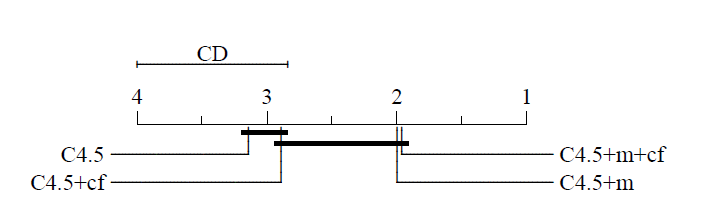
\includegraphics[width=\textwidth]{Figuras/cdp.png}
%     \caption[Critical Difference Plots]{Critical Difference Plot que compara cuatro clasificadores.}
%     \label{fig:CDP}
% \end{figure}



\subsubsection{Votación y conteo de borda} \label{sec:Votacion}

Si tenemos más de tres poblaciones a comparar, para decidir cuál de ellas tiene una mediana, por ejemplo, mayor, tendríamos que hacer comparaciones uno a uno de todos los pares poblacionales. Realizando seis pruebas de Wilcoxon en total. Después de esto, nos quedaríamos con un conjunto de \emph{victorias} de ciertas poblaciones sobre otras y, posiblemente, algunos resultados no significativos ¿Cómo escogeríamos a un ganador desde esta situación?

No siempre es el caso que podemos establecer sólo un orden parcial en el conjunto de votaciones. En particular, una elección que se puede tomar es el llamado \textbf{conteo de borda}. En este se cuentan \emph{victorias} totales que tiene una población sobre otra para determinar el ganador. Usaremos esta manera de indicar cuando un algoritmo tiene mejor desempeño que otro. De la misma forma que en la discusión de la Sección \ref{sec:FWER_Bonferroni}, un análisis que busque responder preguntas más específicas se puede derivar de los resultados de este trabajo. 








%%%%%%%%%%%%%%%%%%%%%%%%%%%%%%%%%%%%%%%%%%%%%%%%%%%%%%%%%%%%%%%%%%%%%%%%%
%                          Modelado                                     %
%%%%%%%%%%%%%%%%%%%%%%%%%%%%%%%%%%%%%%%%%%%%%%%%%%%%%%%%%%%%%%%%%%%%%%%%%
% \section{\textcolor{Azul}{Sección en color azul}}
% \subsection{SubSección}
% Antes de comenzar, se definen  en la Tabla ~\ref{tab:Tabla} los parámetros y variables utilizadas

% %%%%%%%%Tabla Nombres de parámetros
% \begin{table}[ht]                             %Inicia el entorno table debajo del texto
% \centering\                                     %   centra la Tabla
% \begin{tabular}{||c | c ||}                     %inicia entorno tabular con doble línea en las orillas, 2 columnas con el contenido centrado (c)
% \hline                                          %inserta línea horizontal
% \hline
% Nombre Parámetro/Variable & Símbolo\\
% \hline
% \hline
% Masa del péndulo & $m$ \\
% \hline
% Masa del carro & $M$\\
% \hline
% Distancia del eje de giro al centro de masa & $l$ \\
% \hline
% Aceleración gravitatoria & $g$ \\
% \hline
% Momento de inercia péndulo respecto del eje de giro& $J$ \\
% \hline
% Ángulo del péndulo respecto del eje vertical & $\theta$\\
% \hline
% Velocidad angular del péndulo & $\dot{\theta}$, $\omega$\\
% \hline
% Distancia del carro respecto al centro del riel & x\\
% \hline
% Velocidad del carro & $\dot{x}$, $v$\\
% \hline
% \hline
% \end{tabular}
% \caption[Parámetros dinámicos del carro-péndulo]{\textbf{Parámetros dinámicos del carro-péndulo} - Estos son los valores de parámetros utilizados en el diseño y las simulaciones, corresponden a los valores reales.}
% \label{tab:Tabla}                              %etiqueta para referencia
% \end{table}

% \blindtext


%%%%%%%%%%%%%%%%%%%%%%%%%%%%%%%%%%%%%%%%%%%%%%%%%%%%%%%%%%%%%%%%%%%%%%%%%
%                          SubSección
%%%%%%%%%%%%%%%%%%%%%%%%%%%%%%%%%%%%%%%%%%%%%%%%%%%%%%%%%%%%%%%%%%%%%%%%%

